%===============================================================================
% Brno University of Technology
% Faculty of Information Technology
% Academic year: 2018/2019
% Bachelor thesis: Monitoring Pedestrian by Drone
% Author: Vladimir Dusek
%===============================================================================

\chapter{Experimenty}
\label{chap_6}

Vyhodnocení přesnosti detektoru bylo provedeno metrikou Averige Precision (AP). Jedná se o~způsob, který se používá na soutěžích Pascal VOC Challenge. Rozhodnutí, jestli detekce byla správná či nikoliv, se uskutečňuje pomocí metody Intersection over Union (IoU). Je spočítán podíl průniku a sjednocení predikované oblasti a oblasti skutečně anotované. Oblast predikovaná je označena $A$ a oblast skutečně anotovaná $B$. Výpočet pak vypadá následovně.

\begin{equation}
    IoU(A, B) = \frac{A \cap B}{A \cup  B}
\end{equation}

Pokud podíl vyjde vyšší než~0,5 je detekce považována za úspěšnou a označena jako skutečně pozitivní (\textit{true positive}). V~opačném případě je označena za falešně pozitivní (\textit{false positive}). Případ, kdy není anotovaný objekt nalezen vůbec, je označen jako falešně negativní (\textit{false negative}). Z~těchto ukazatelů lze vypočítat metriky \textit{precision} a \textit{recall}. AP potom shrnuje tvar $precision\,/\,recall$ křivky~\cite{paperAP}.

\begin{equation}
    precision = \frac{true \: positives}{true \: positives + false \: positives}
\end{equation}

\begin{equation}
    recall = \frac{true \: positives}{true \: positives + false \: negatives}
\end{equation}

Zhodnocení úspěšnosti reidentifikace osob a správnosti vykreslených trajektorií bylo provedeno subjektivně po otestování na několika demonstračních videích. Bylo vyhodnoceno, s~čím má algoritmus problémy a kde naopak funguje.

%===============================================================================

\pagebreak

\section{Úspěšnost a rychlost detektoru}
\label{sec_detector_results}

Vyhodnocení přesnosti detektoru bylo měřeno na validační části datasetu SDD (sekce~\ref{sec_dataset}). Přesnost byla měřena na modelech z~finálního třetího trénování, kde se dosáhlo nejnižší validační chyby. Nejvyšší přesnosti AP dosáhl model po 40.~trénovací epoše a to sice~58,6\,\%.

\begin{figure}[H]
    \centering
    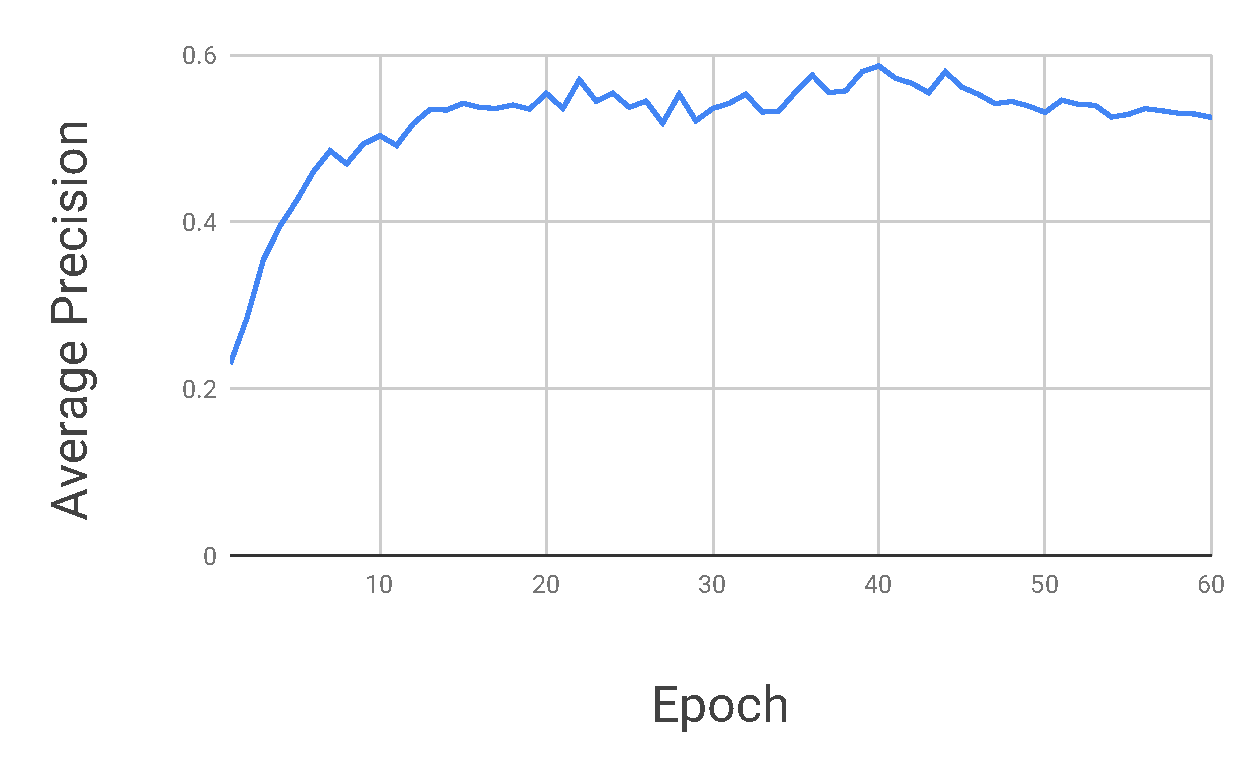
\includegraphics[width=.65\textwidth]{t3-ap.pdf}
    \caption[Přesnost natrénovaného modelu]{Vývoj přesnosti AP v~závislosti na množství odtrénovaných epoch.}
\end{figure}

Měření rychlosti modelu probíhalo na operačním systému Ubuntu~18.04 s~interpretem Pythonu verze~3.7.3 a knihovnou Tensorflow verze~1.13. Procesor Intel Core i7~8565U Whiskey Lake potřeboval na zpracování jednoho snímku kolem 3~sekund. Zpracování obrázku s~akcelerací pomocí grafické karty nVIDIA GeForce GTX~1070 trvalo zhruba 0,1~vteřiny.

\begin{figure}[H]
    \centering
    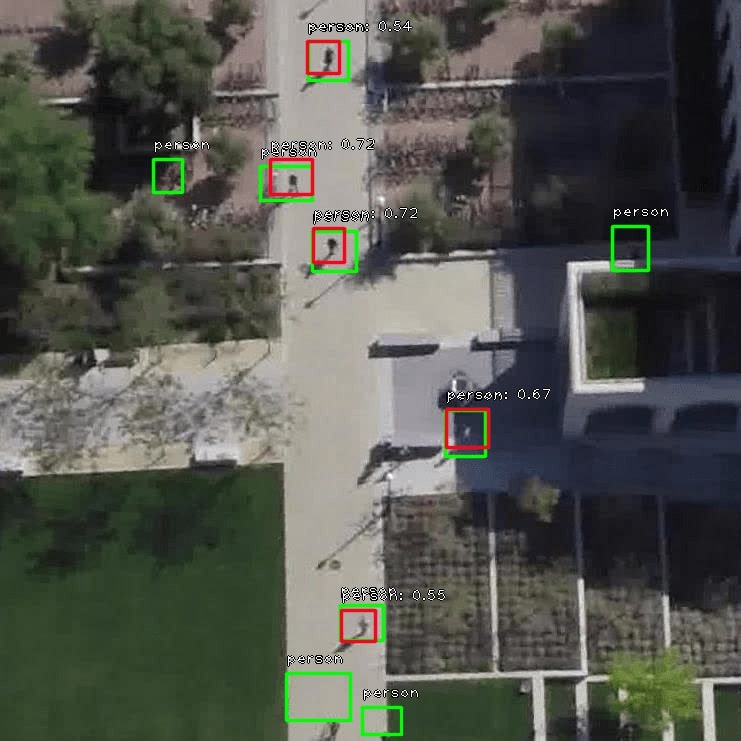
\includegraphics[width=.49\textwidth]{evaluated-1.jpg}\hfill
    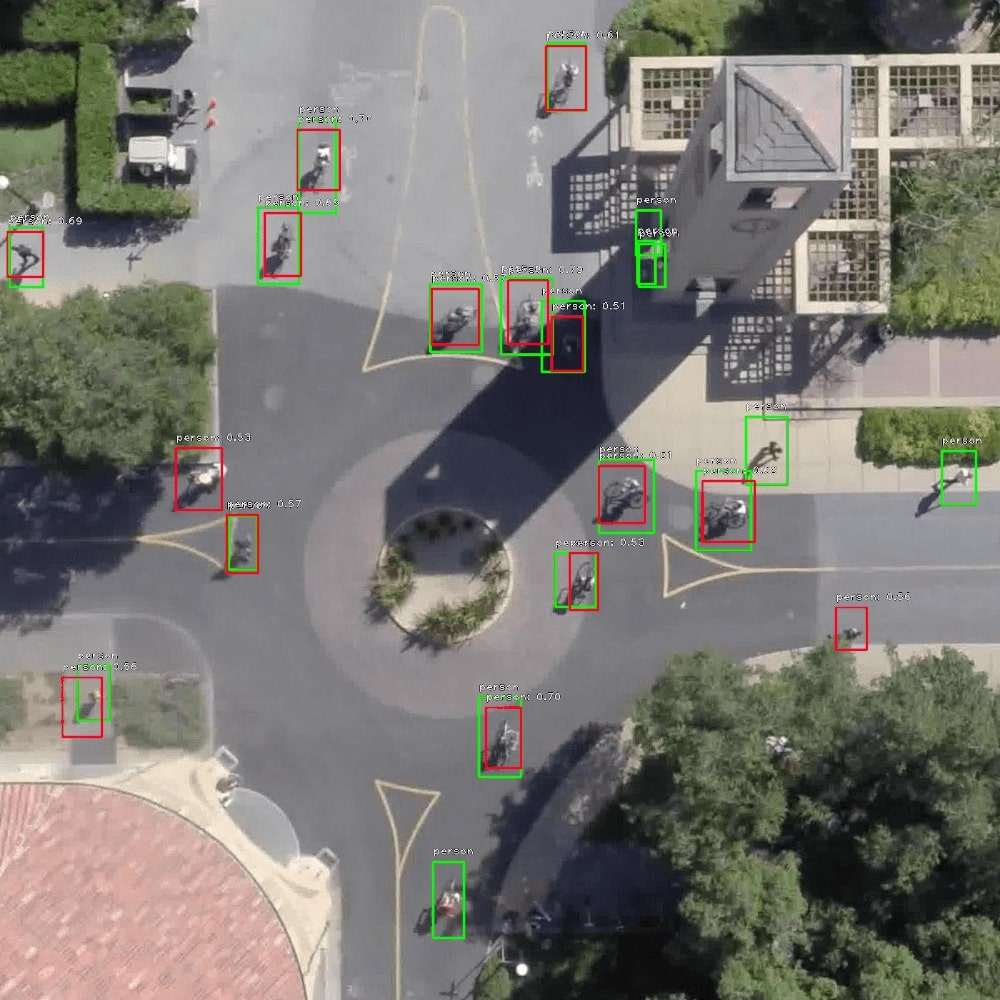
\includegraphics[width=.49\textwidth]{evaluated-3.jpg}
    \caption[Ukázka z~vyhodnocování přesnosti modelu]{Ukázka z~vyhodnocování přesnosti na validačních datech. Zeleně jsou vyznačeni skutečně anotovaní lidé, červeně rozpoznaní. Je zřejmé, že někde nejsou anotace vyznačeny přesně, jak bylo popsáno v~sekci~\ref{sec_training_process}. To kazí celkovou naměřenou přesnost.}
\end{figure}

\begin{figure}[H]
    \begin{tabular}{cc}
        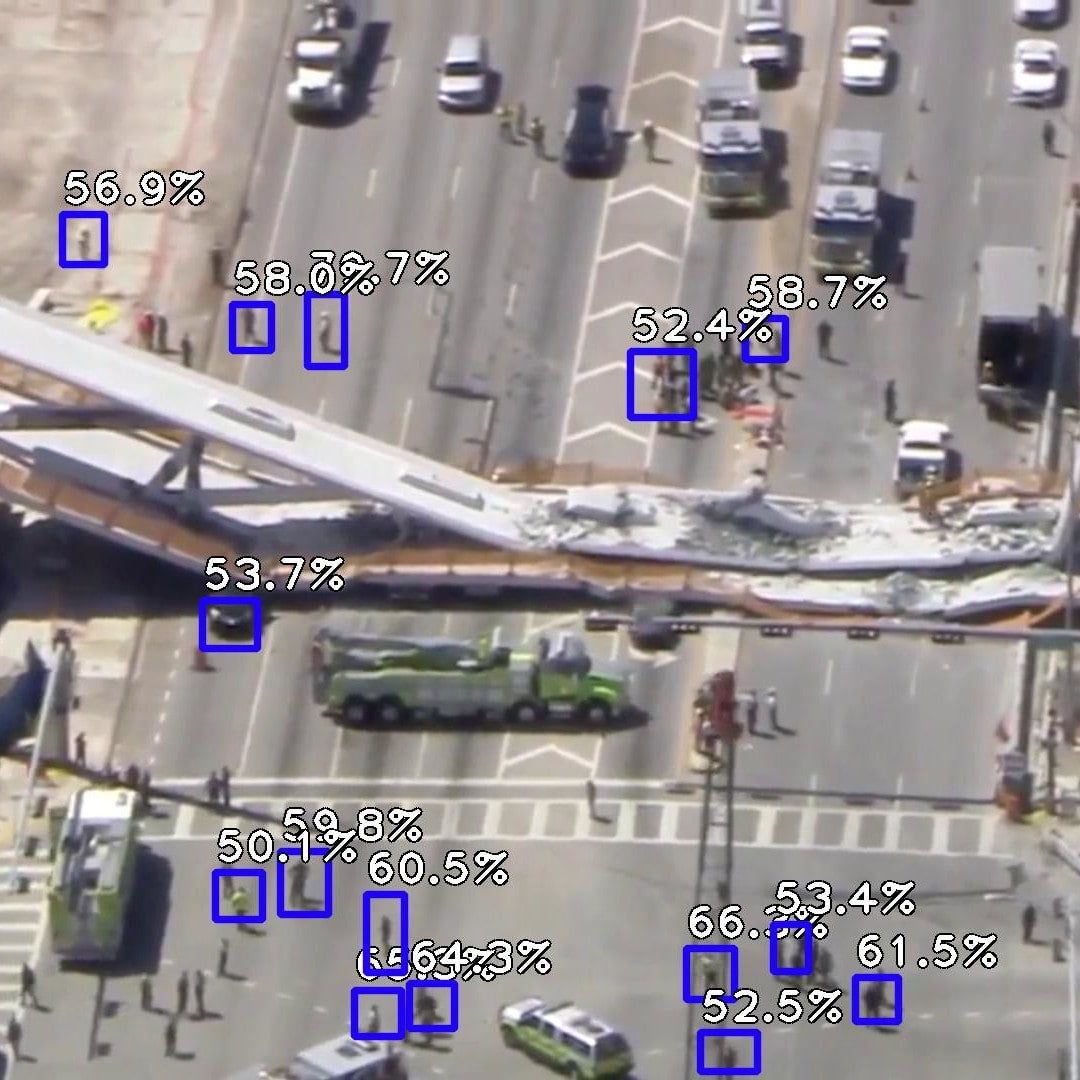
\includegraphics[width=.49\textwidth]{t3-t1.jpg} &
        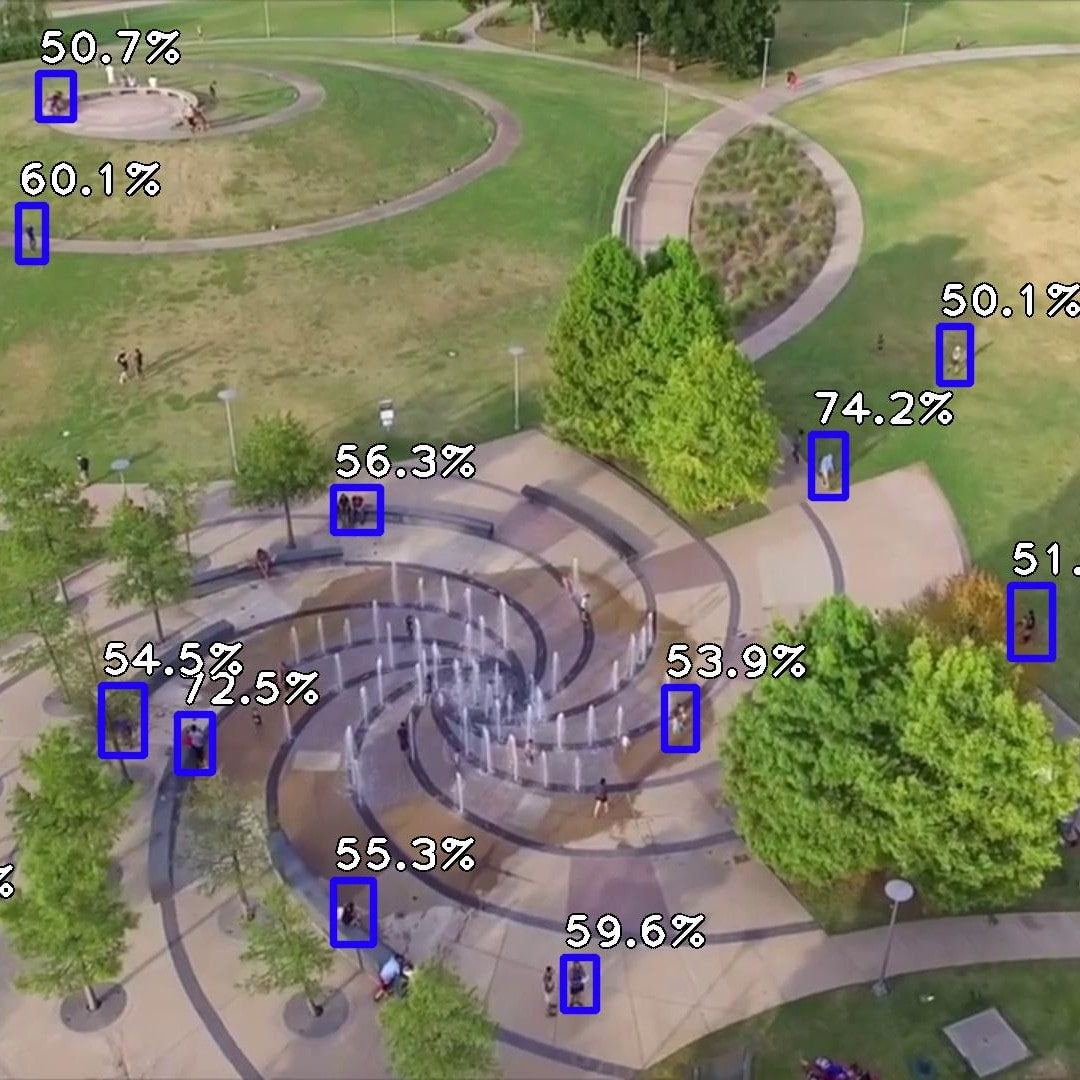
\includegraphics[width=.49\textwidth]{t3-t2.jpg} \\
        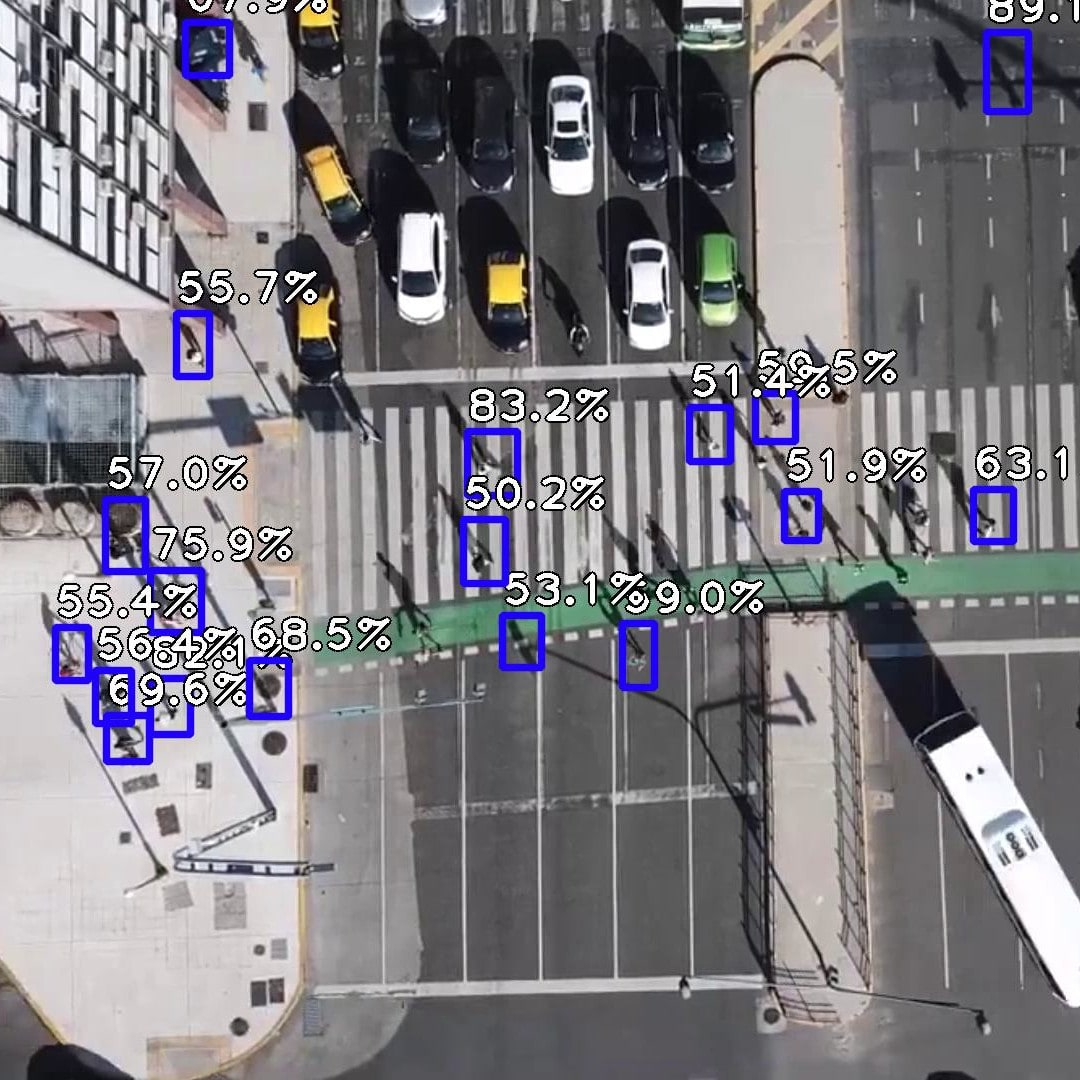
\includegraphics[width=.49\textwidth]{t3-t3.jpg} &
        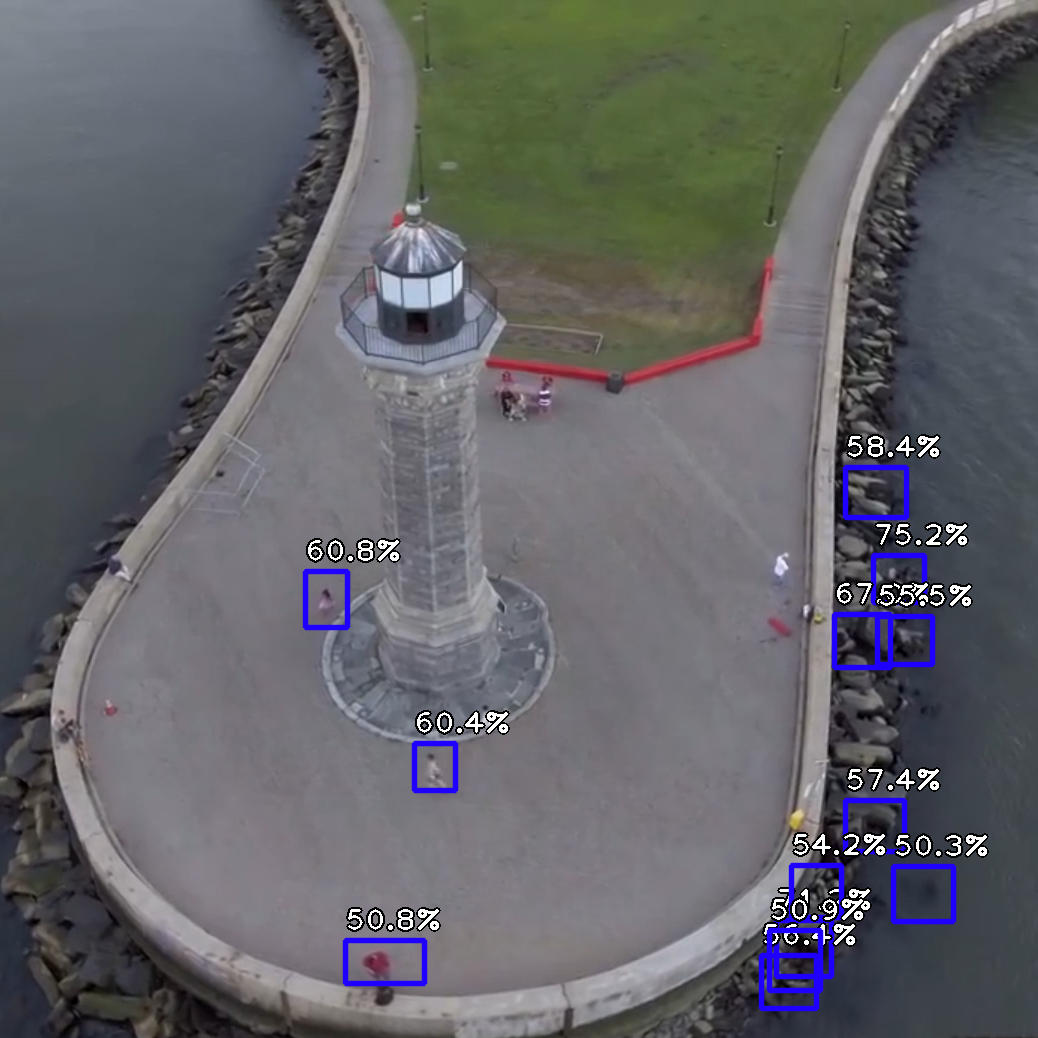
\includegraphics[width=.49\textwidth]{t3-t4.jpg} \\
    \end{tabular}
    \caption[Ukázky detekce lidí na testovacích obrázcích]{Ukázky detekce lidí na testovacích obrázcích, které nebyly součástí původního datasetu. Je zřejmé, že detektor všechny osoby nedetekuje a zároveň ho některé objekty dokáží zmást. Obrázky jsou převzaty z~videí na Youtube.\protect\footnotemark}
\end{figure}

\footnotetext{\url{https://youtu.be/zJq5_7Au13o}, \url{https://youtu.be/7ns6fFhahbw}, \url{https://youtu.be/O9MOb65LVL0}, \url{https://youtu.be/HiZXABMNCUY}}

%===============================================================================

\section{Úspěšnost reidentifikace lidí}
\label{sec_reidentification_results}

Vyhodnocení úspěšnosti reidentifikace lidí a zakreslení správnosti jejich trajektorií probíhalo na záběrech z~validační části použitého datasetu a na pořízených záznamech z~dronu DJI Spark z výšky 35\,m. Z~datasetu byly vybrány takové záběry, kde je možnost reidentifikace aspoň trochu možná, tedy spíše záběry v~lepší kvalitě a pořízené z~nižší výšky. Dataset jinak obsahuje záběry z~velmi vysoké výšky, případně v~nízké kvalitě, kde je v~podstatě člověk viděn pouze jako tmavá čmouha. Tam pochopitelně není možné od sebe jednotlivé lidi rozlišit.

%-------------------------------------------------------------------------------

\subsection*{Scéna Coupa}

\begin{figure}[H]
    \begin{tabular}{cc}
        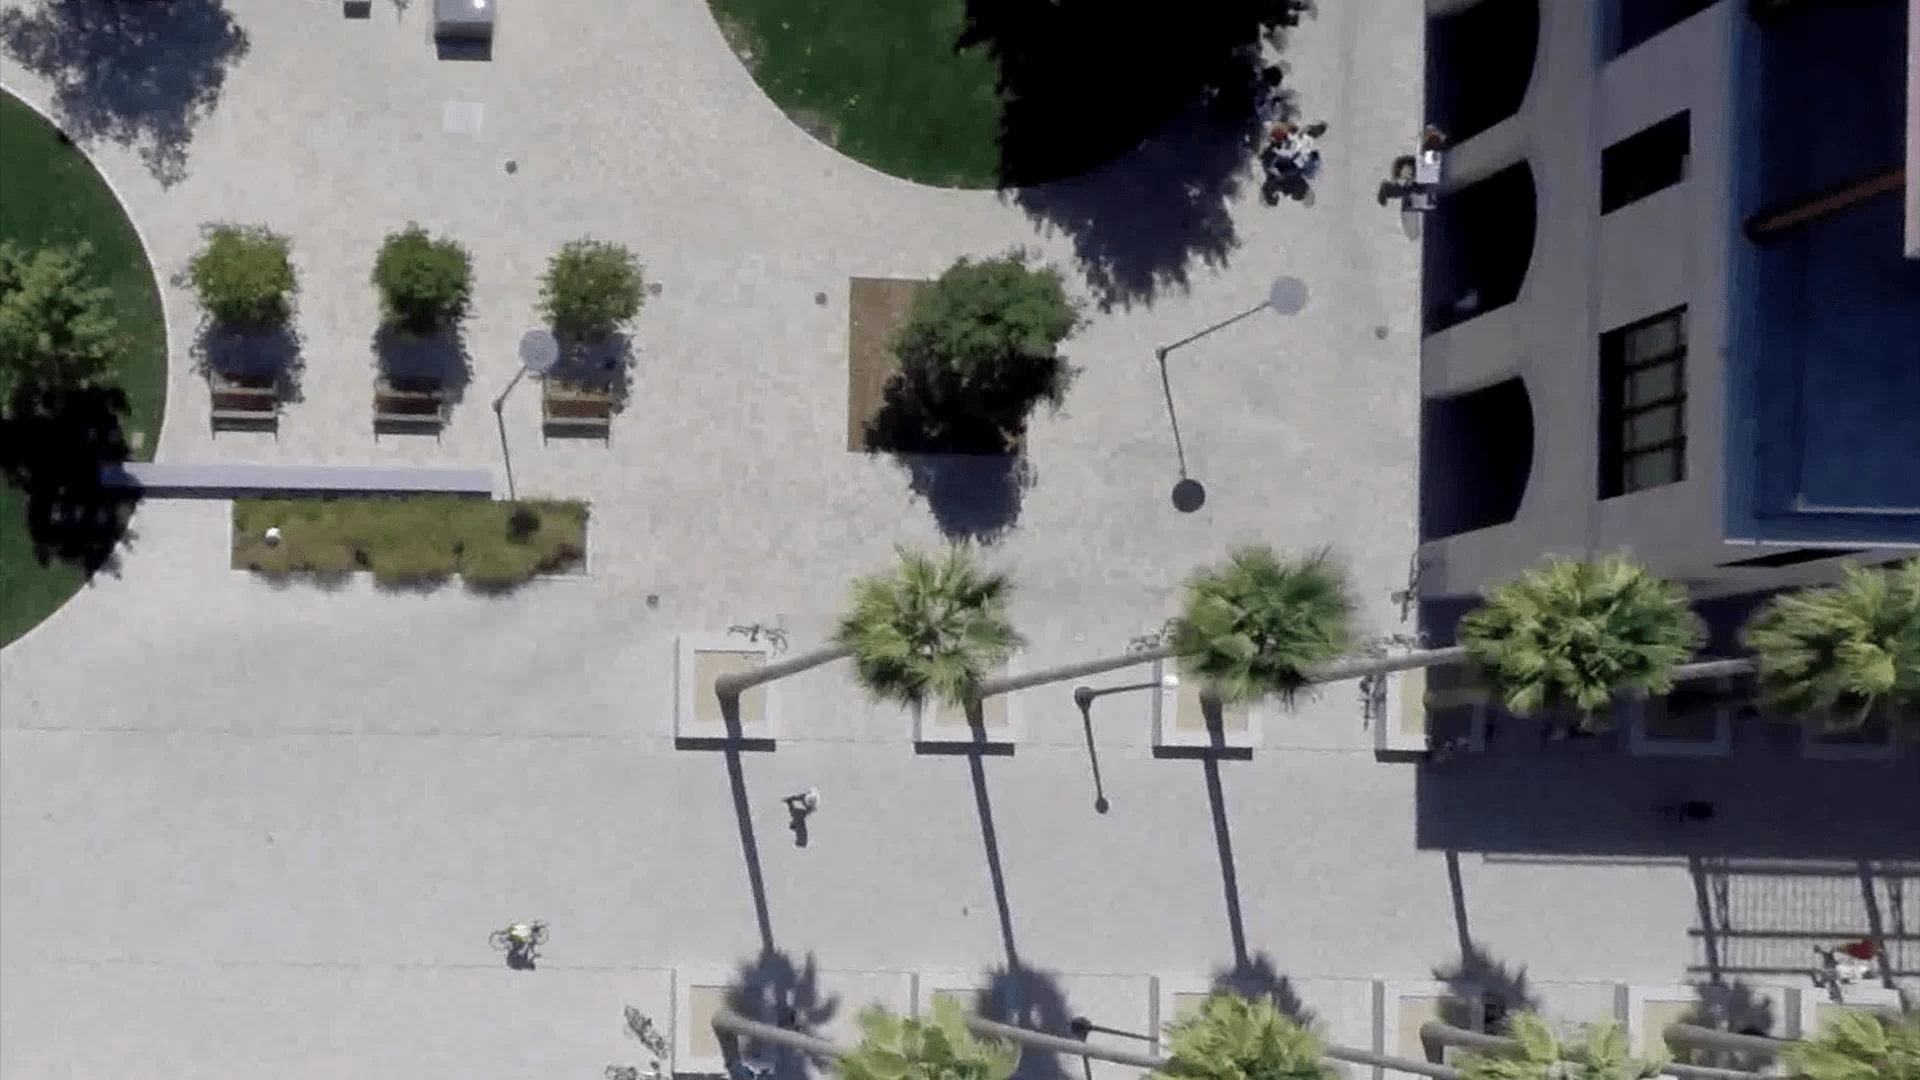
\includegraphics[width=.49\textwidth]{res-coupa-1.jpg} &
        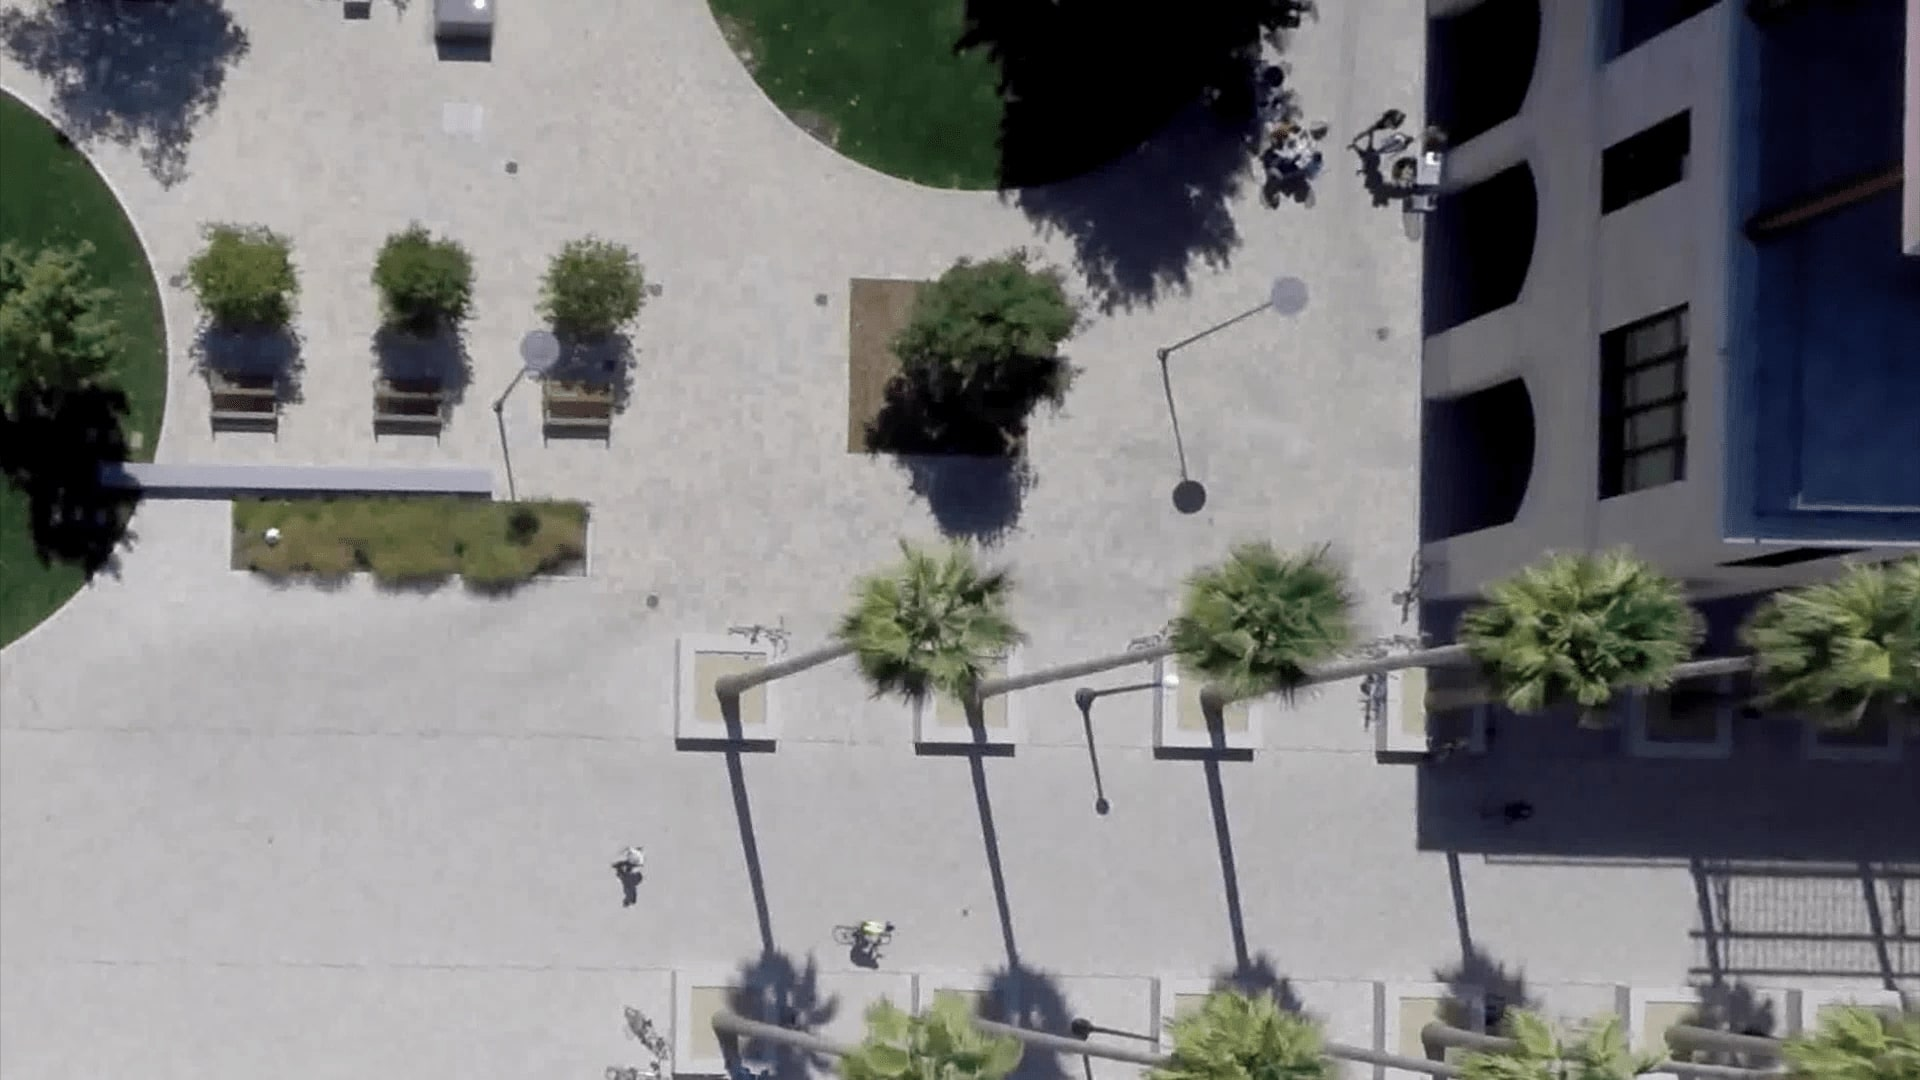
\includegraphics[width=.49\textwidth]{res-coupa-2.jpg} \\
        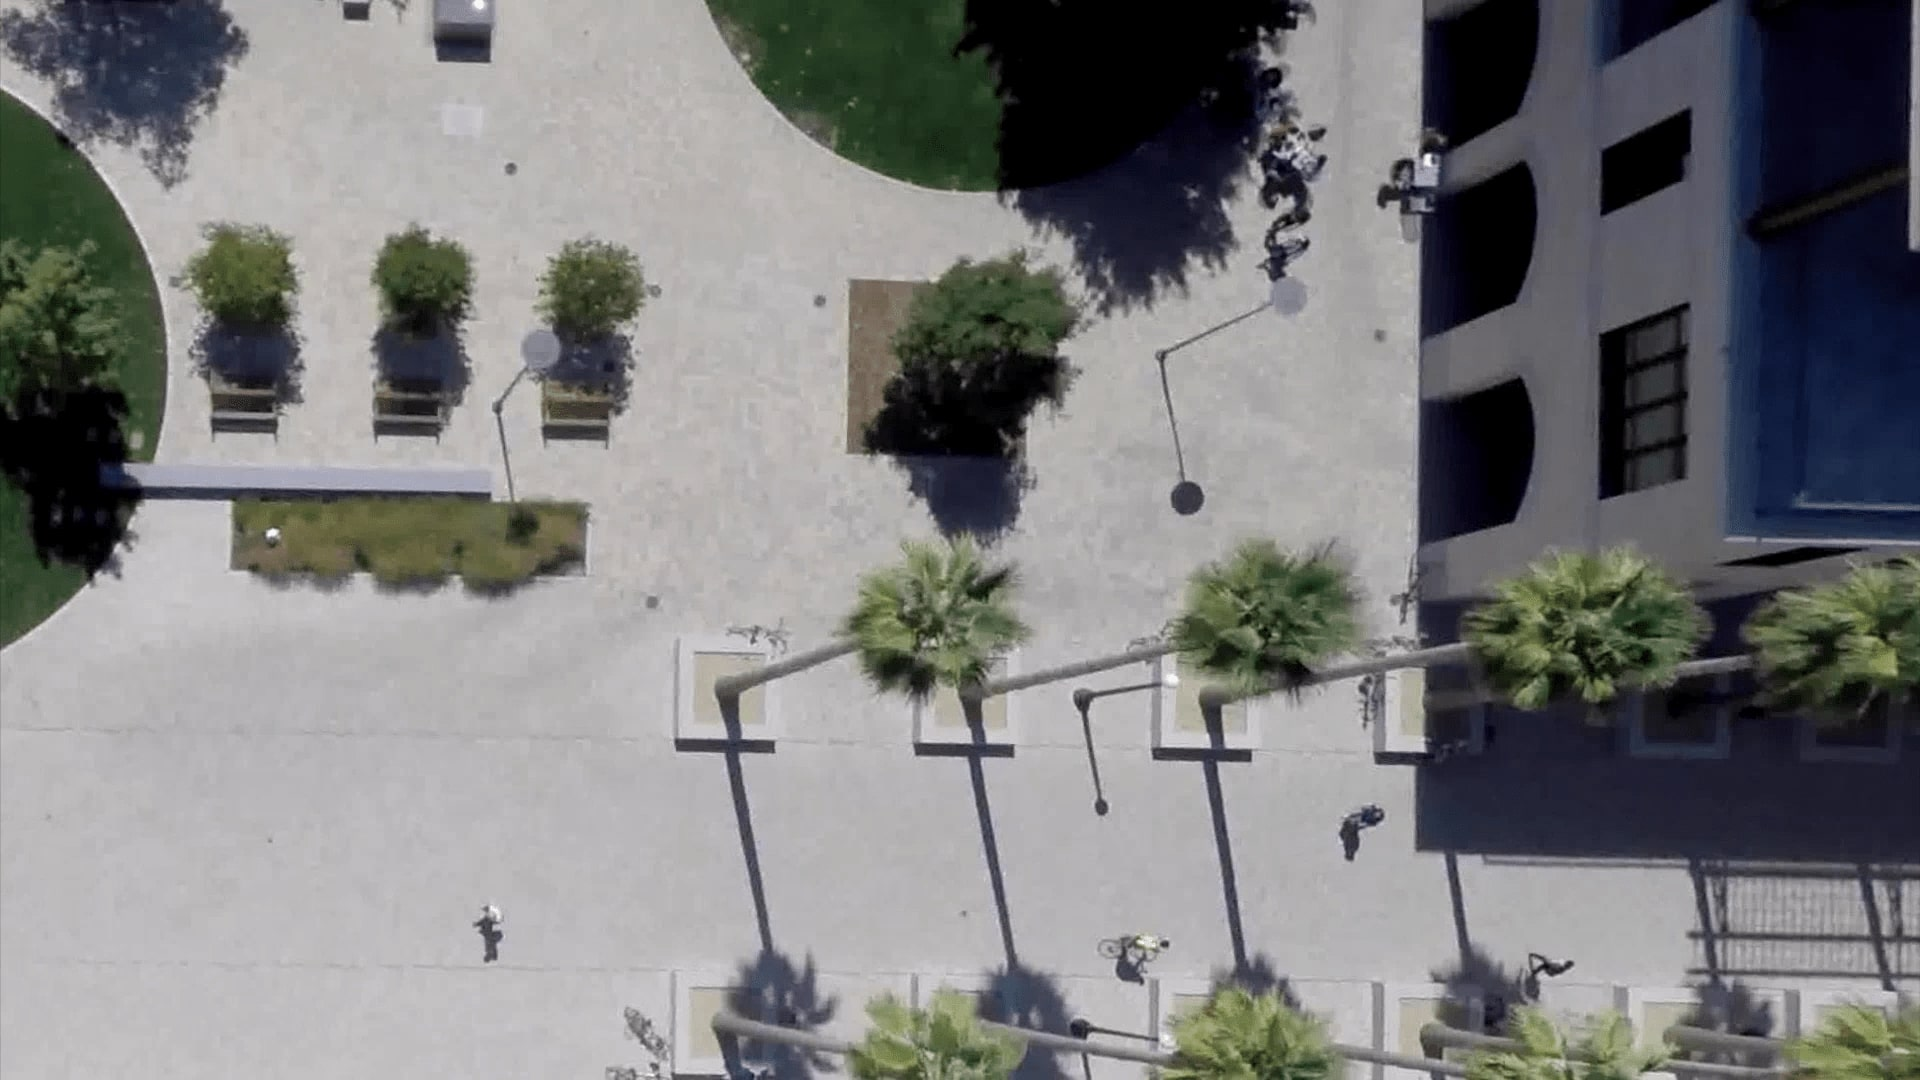
\includegraphics[width=.49\textwidth]{res-coupa-3.jpg} &
        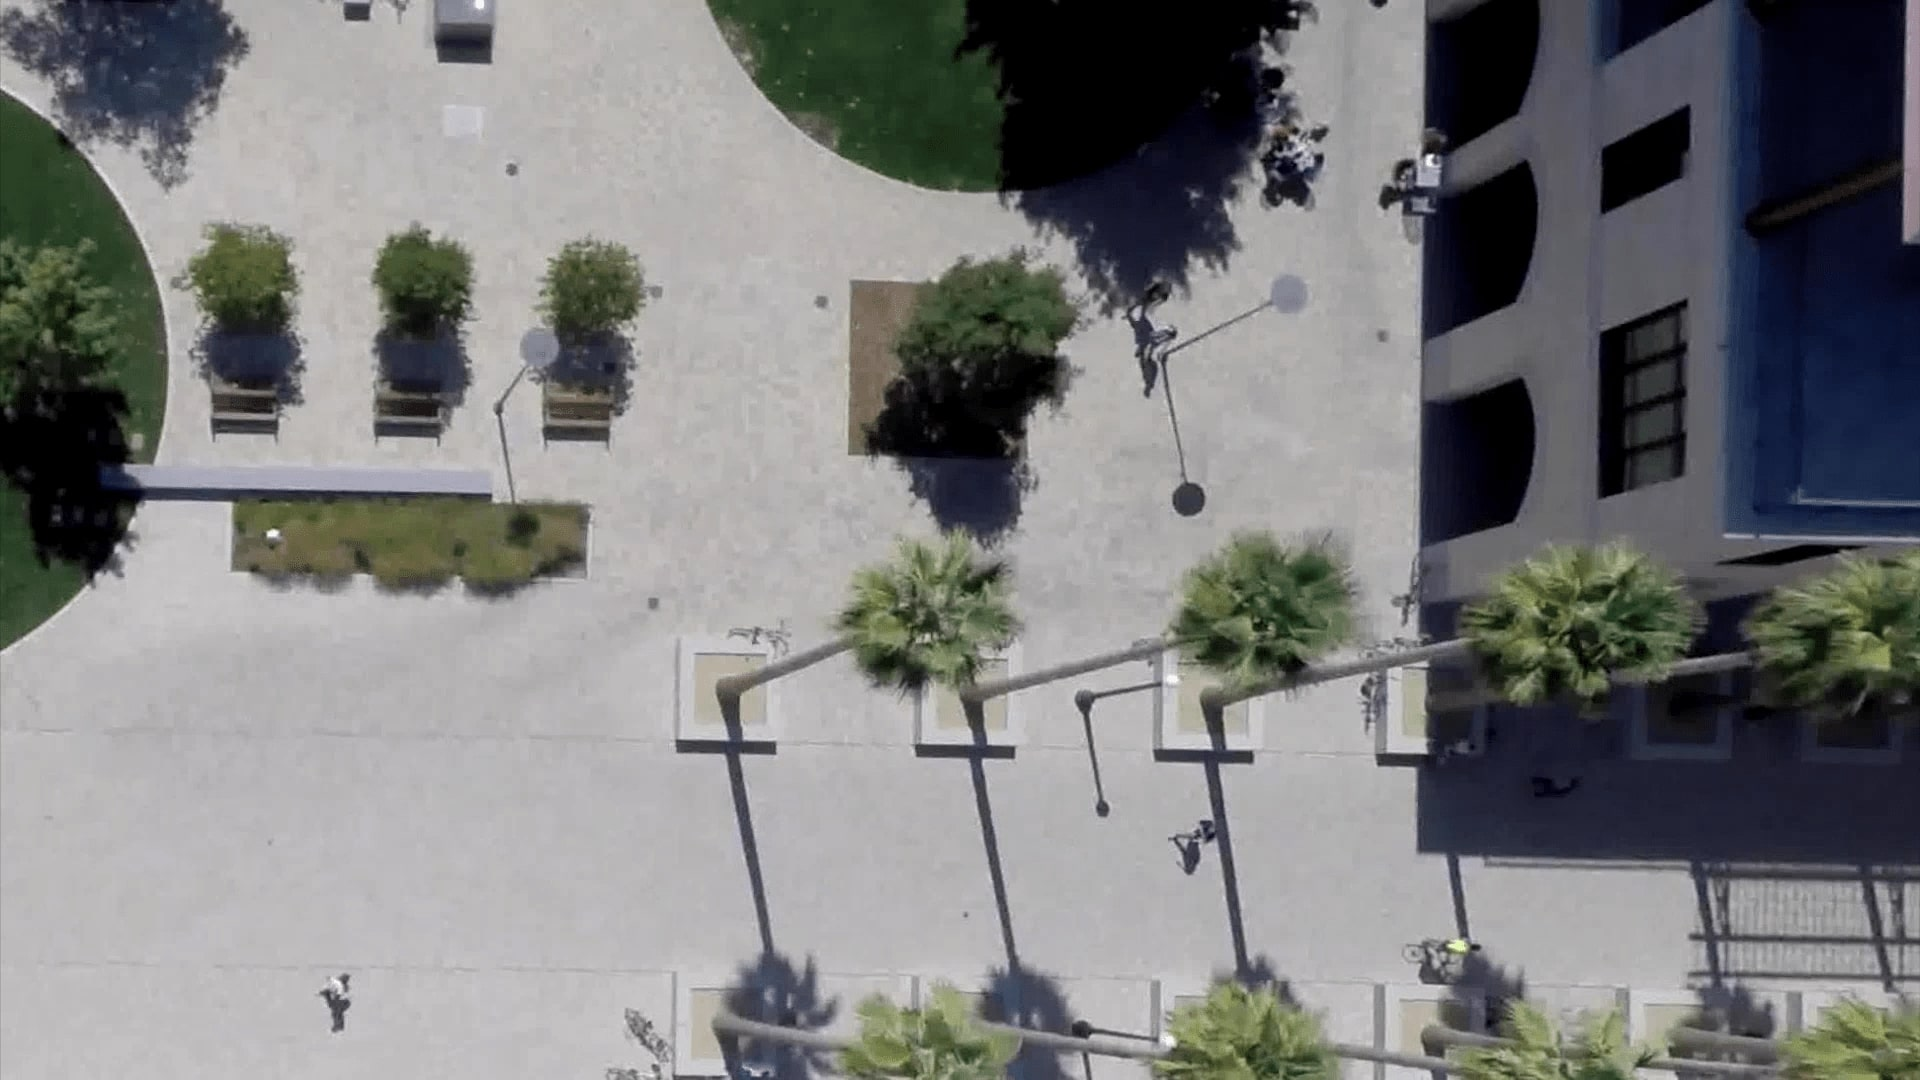
\includegraphics[width=.49\textwidth]{res-coupa-4.jpg} \\
    \end{tabular}
    \caption[Otestování algoritmu na scéně Coupa]{Vstupní 10~vteřinové video ze scény Coupa. V~pravé horní části obrazu se nachází po celou dobu několik sedících osob. V~průběhu kolem nich projde další dvojice osob. V~dolní části se pak pohybuje asi čtveřice osob, kdy jedna z~nich se v~záběru objeví až později. V~pravém dolním rohu odchází ze záběru dvojice osob.}
\end{figure}

\begin{figure}[H]
    \centering
    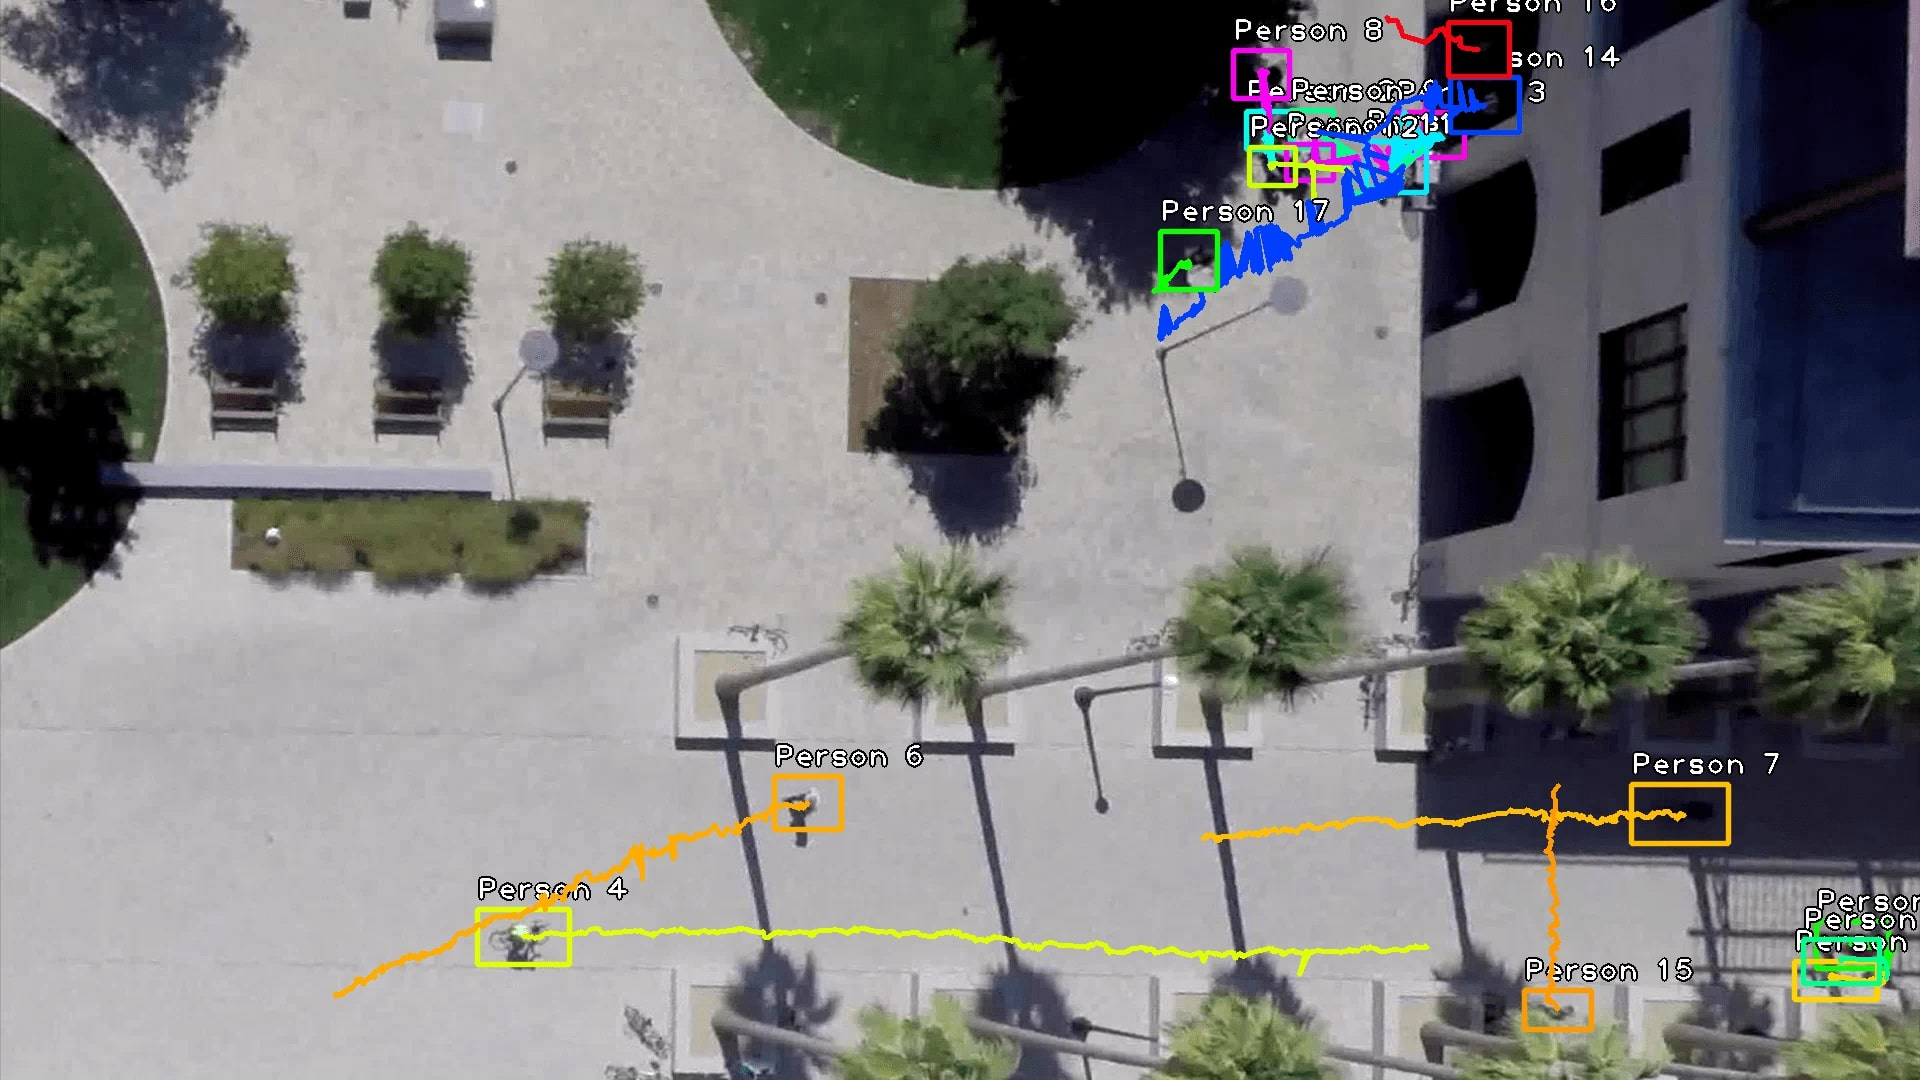
\includegraphics[width=.92\textwidth]{res-coupa-panorama.jpg}
    \caption[Výsledná mapa s~trajektoriemi osob ze scény Coupa]{Výsledná mapa s~trajektoriemi osob ze scény Coupa. }
\end{figure}

Pravý horní roh způsobil velký zmatek. Dvojice chodců, která procházela kolem skupinky sedících lidí, nebyla dostatečně rozlišena. Procházeli velmi blízko sebe a díky tomu, že není nijak vyřešeno oříznutí pozadí chodce a histogram je počítán pro celou výseč, je výsledek takto špatný. Vektory příznaků si jsou příliš podobné. Dolní část obrazu dopadla o~poznání lépe. Všem 4~osobám byly trajektorie vykresleny správně. Osoby se potkaly, ale pomocí vektoru příznaků od sebe byly správně rozpoznány. Osoba~7 navíc vyšla ze stínu, algoritmus se přesto zachoval správně. Další problém nastal s~dvojicí osob v~pravém dolním rohu, která byla v~obraze pouze chvilku a procházela přes částečný stín. Osoby nebyly úspěšně reidentifikovány, jejich příznakové vektory se napříč snímky příliš lišily.

%-------------------------------------------------------------------------------

\subsection*{Scéna Little}

\begin{figure}[H]
    \begin{tabular}{cc}
        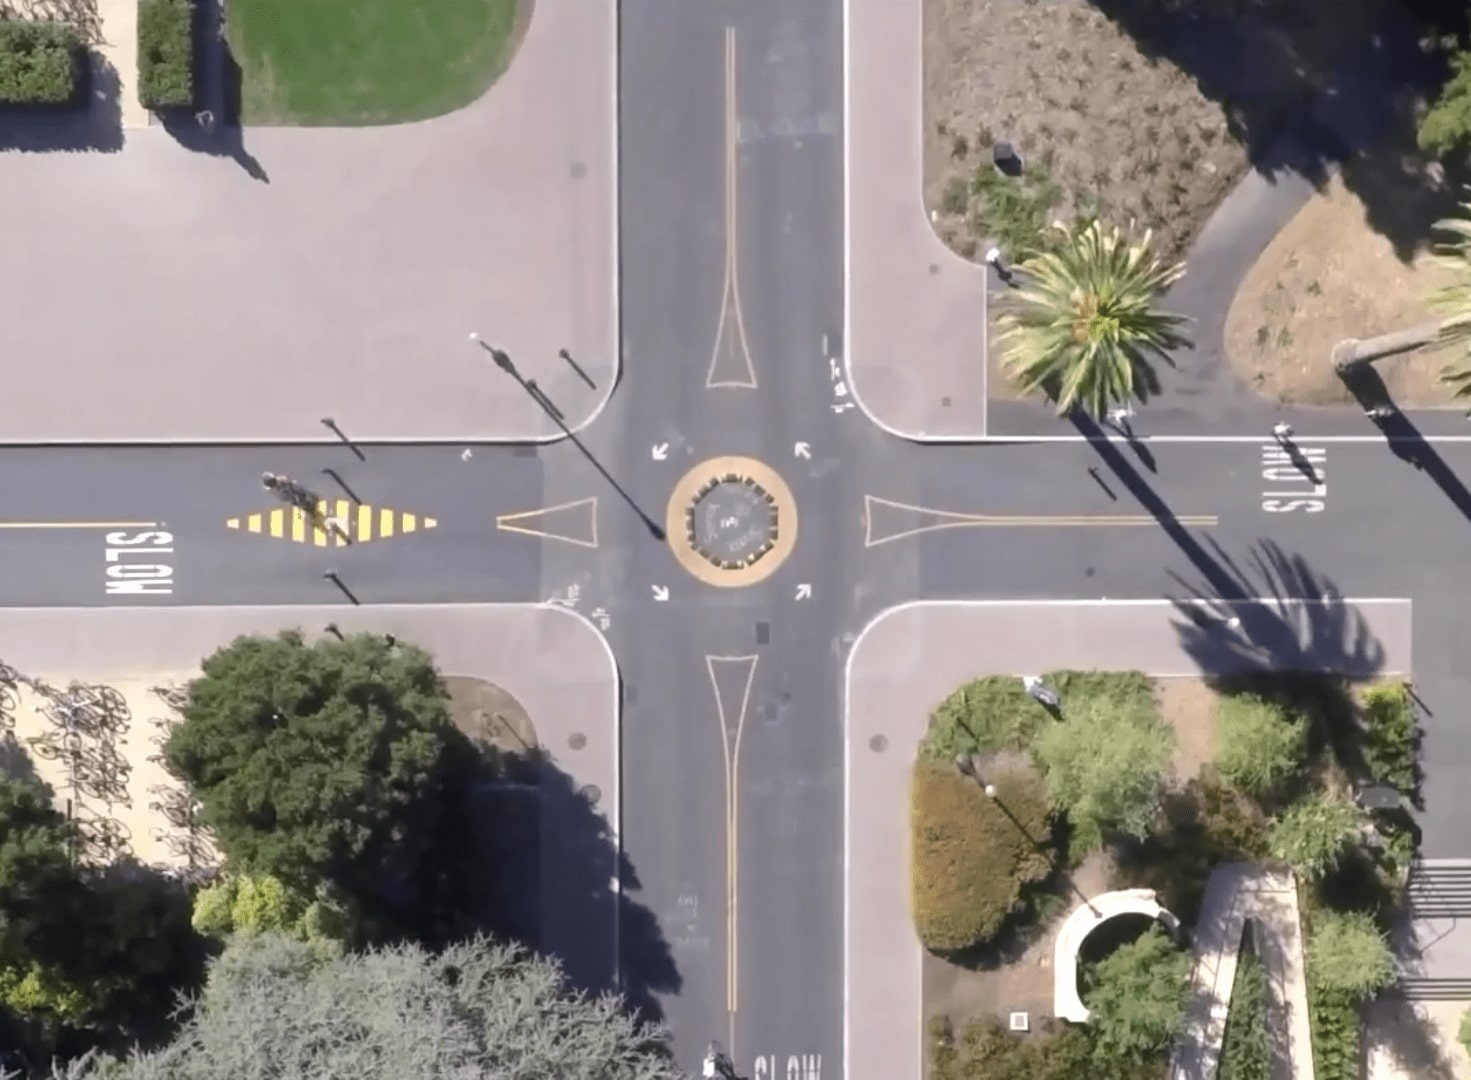
\includegraphics[width=.49\textwidth]{res-little-1.jpg} &
        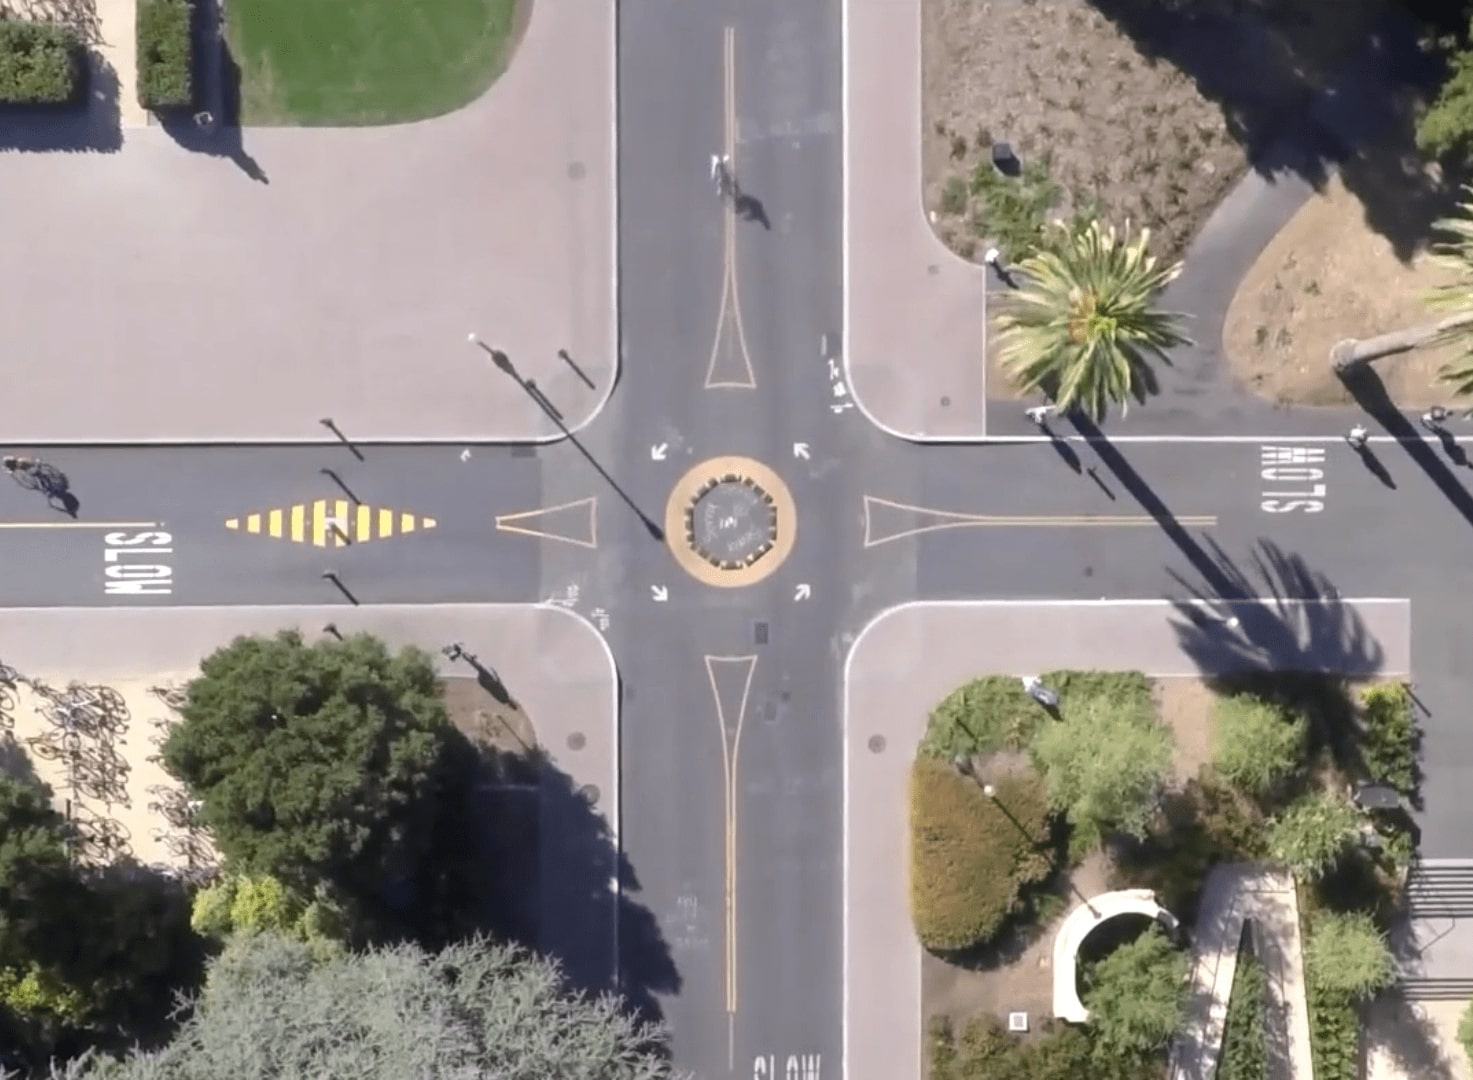
\includegraphics[width=.49\textwidth]{res-little-2.jpg} \\
        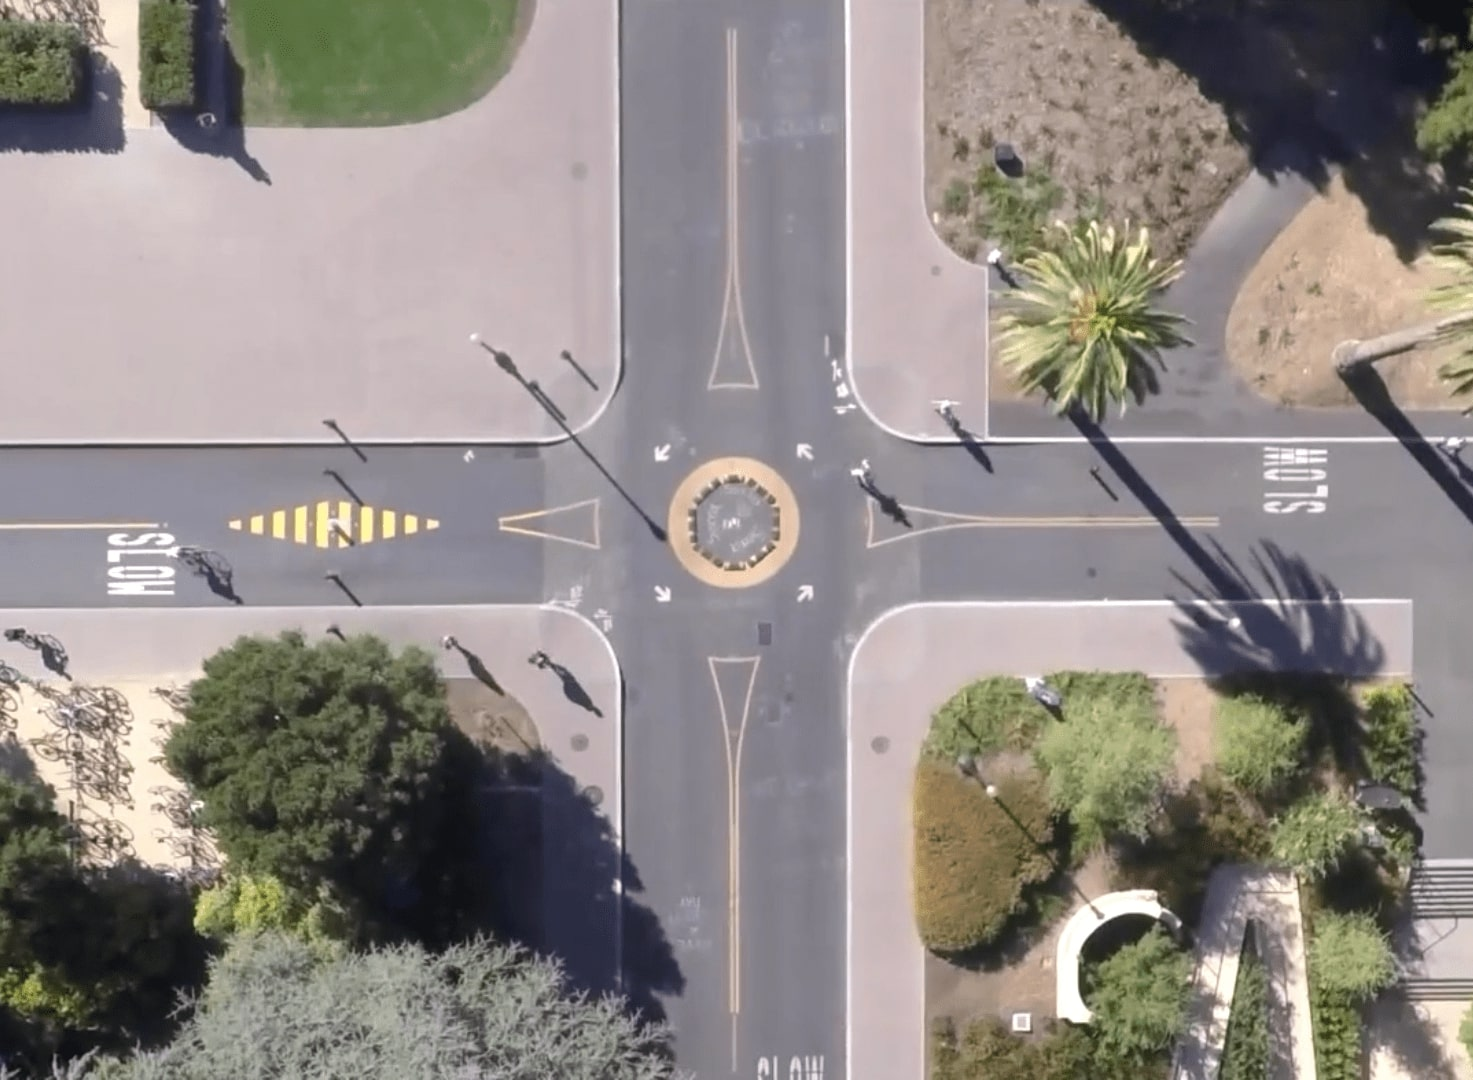
\includegraphics[width=.49\textwidth]{res-little-3.jpg} &
        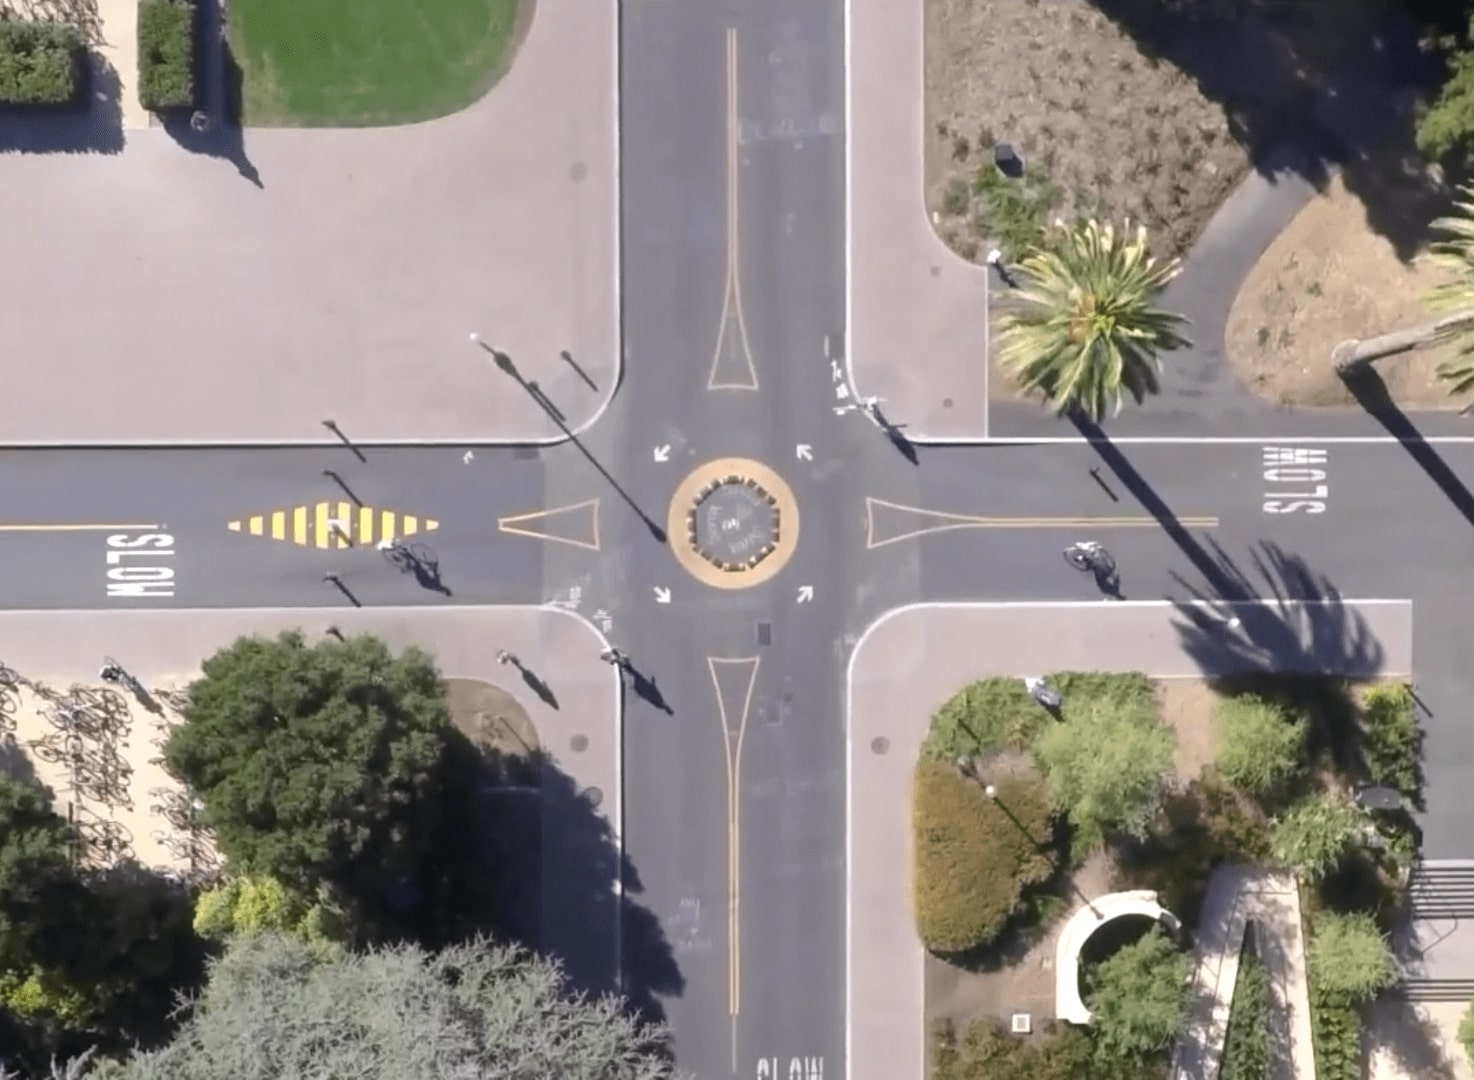
\includegraphics[width=.49\textwidth]{res-little-4.jpg} \\
    \end{tabular}
    \caption[Otestování algoritmu na scéně Little]{Vstupní 7~vteřinové video ze scény Little. V~obrázku se pohybují chodci a cyklisté. Někteří procházejí skrz stíny, pod lehkým zákrytem stromů nebo do záběru vstupují až v~průběhu záznamu.}
\end{figure}

\begin{figure}[H]
    \centering
    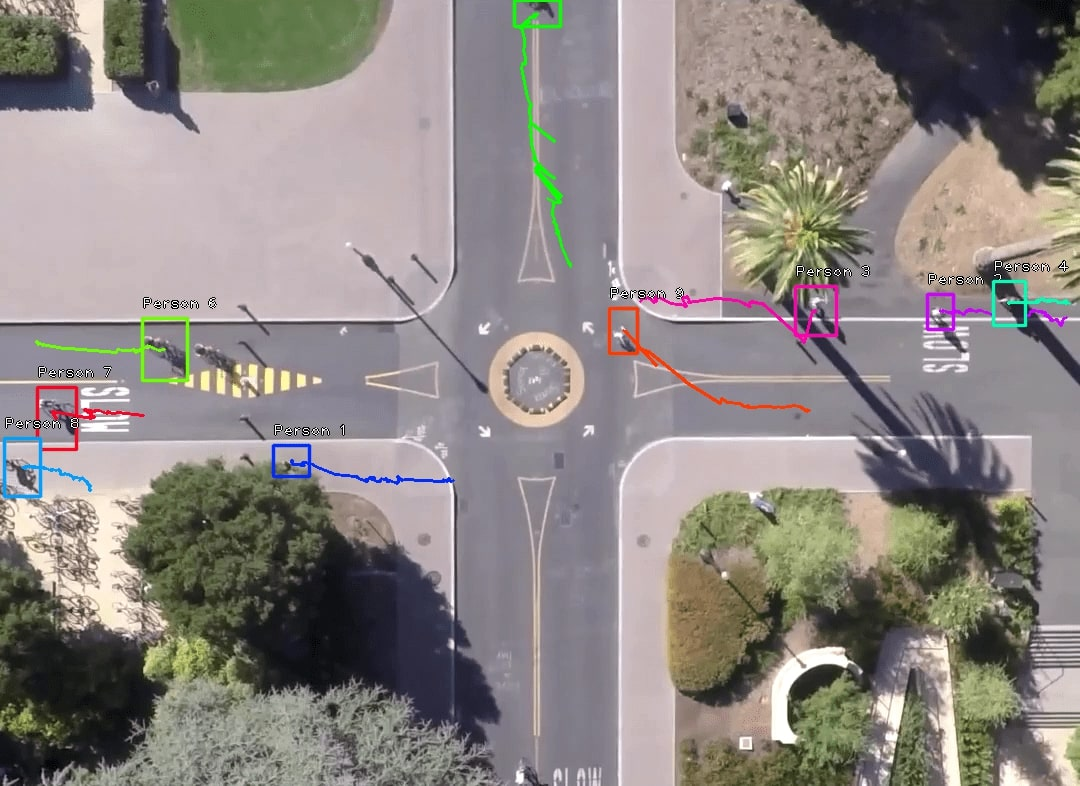
\includegraphics[width=.99\textwidth]{res-little-panorama.jpg}
    \caption[Výsledná mapa s~trajektoriemi osob ze scény Little]{Výsledná mapa s~trajektoriemi osob ze scény Little.}
\end{figure}

Cyklistu~6 síť nerozpoznala ihned, ale až po několika snímcích, proto je jeho výřez vidět dvakrát. Výřez více vpravo je pozice cyklisty v~prvním snímku. Označený výřez vlevo je moment, kdy byl sítí poprvé rozpoznán. Osoby~7,~8 se v~záběru objevily až později a byly správně detekovány a reidentifikovány. Člověk~1 je na počátku schovaný pod stromem, v~záběru se ukáže až v~průběhu videa a je správně rozpoznán. Osoby~2,~4 projdou stínem, přesto jsou správně reidentifikovány. Člověk~3 projde stínem, částečně pod zákrytem stromu a je opět správně rozpoznán. Cyklista~9 se uprostřed křižovatky ztratí, síť ho přestane na několik snímků detekovat. Po jeho zpětném rozpoznání je už považován za jinou osobu, protože se mezitím dostal příliš daleko.

%-------------------------------------------------------------------------------

\subsection*{Scéna Death Circle}

\begin{figure}[H]
    \begin{tabular}{cc}
        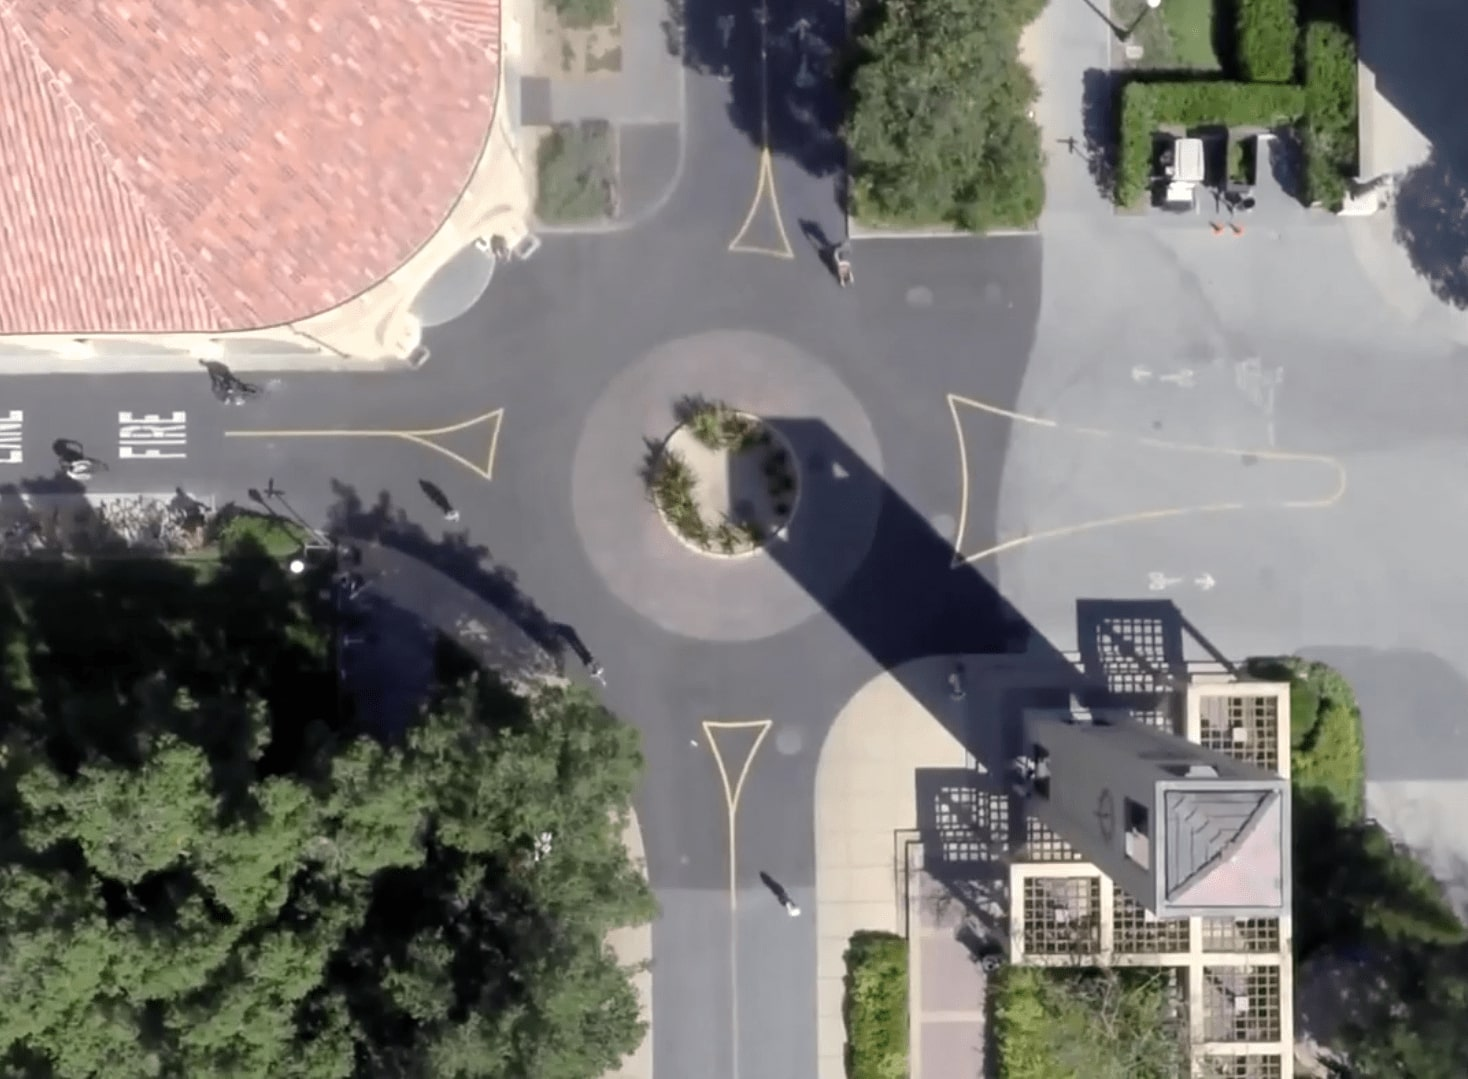
\includegraphics[width=.49\textwidth]{res-death_circle-1.jpg} &
        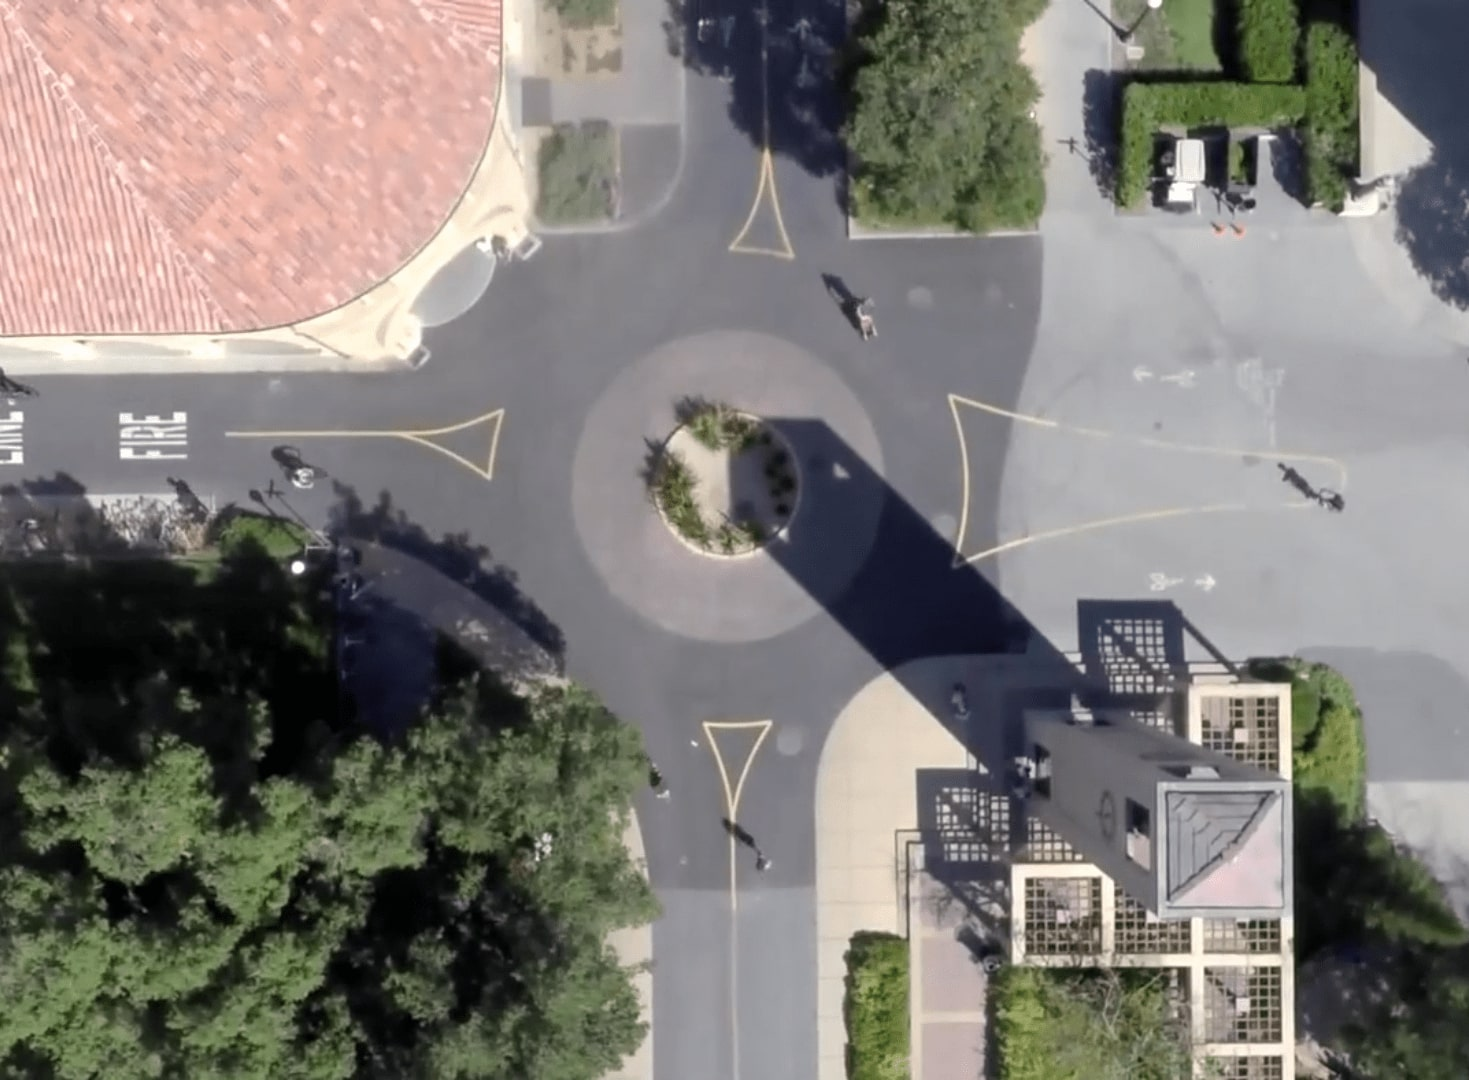
\includegraphics[width=.49\textwidth]{res-death_circle-2.jpg} \\
        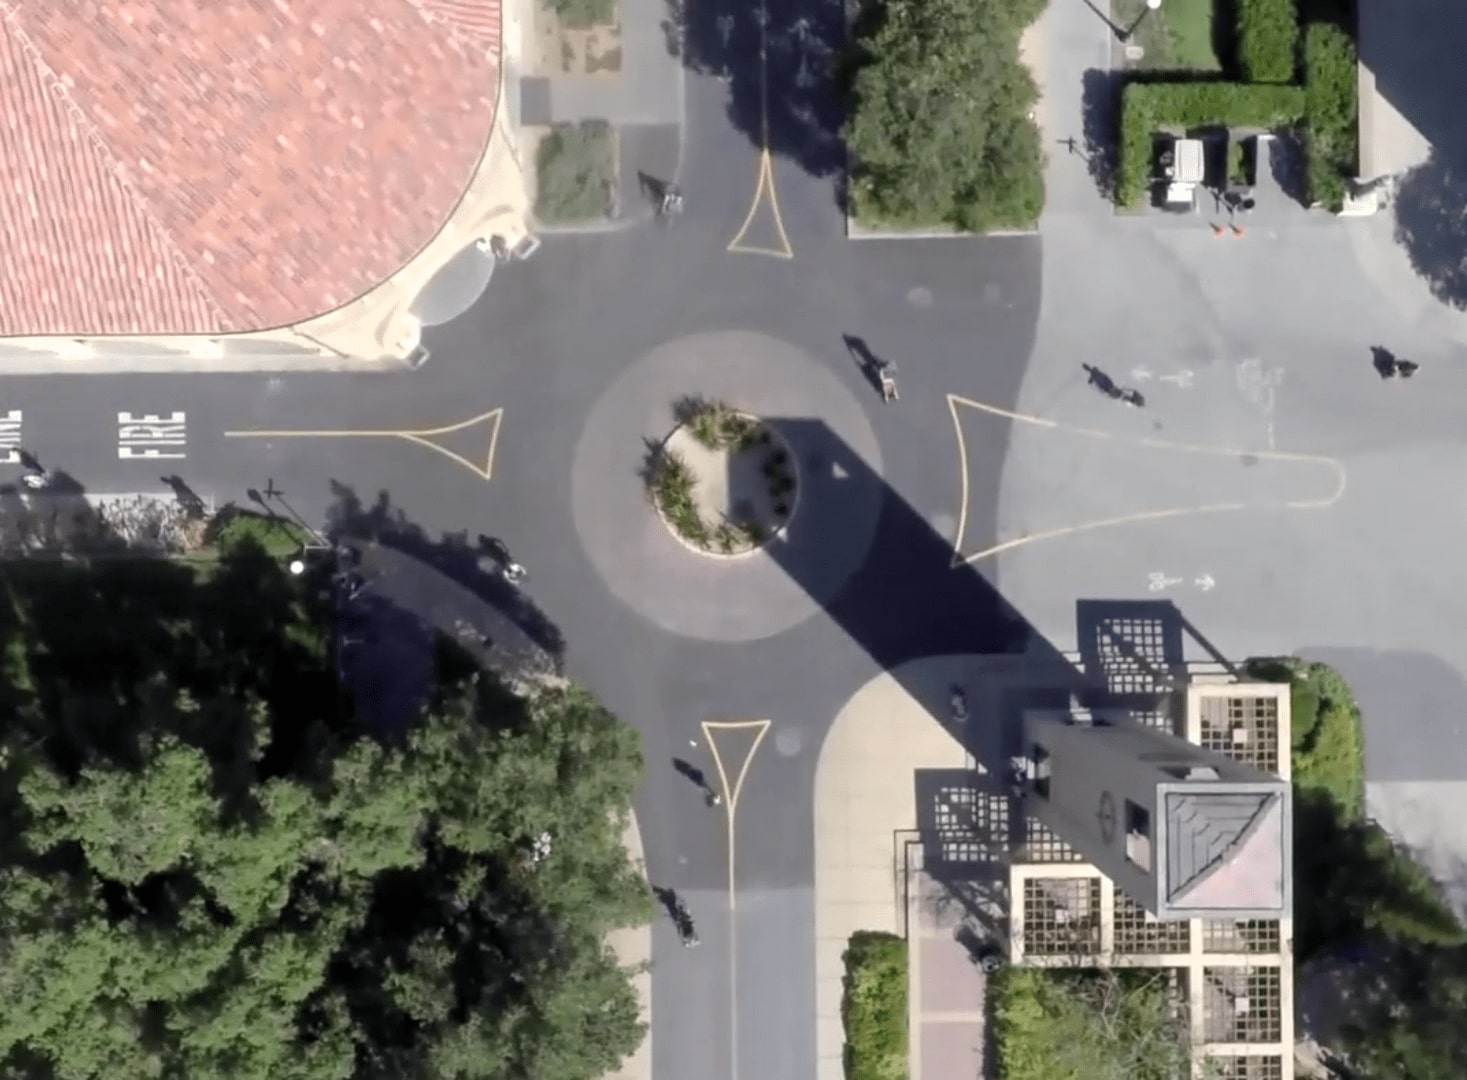
\includegraphics[width=.49\textwidth]{res-death_circle-3.jpg} &
        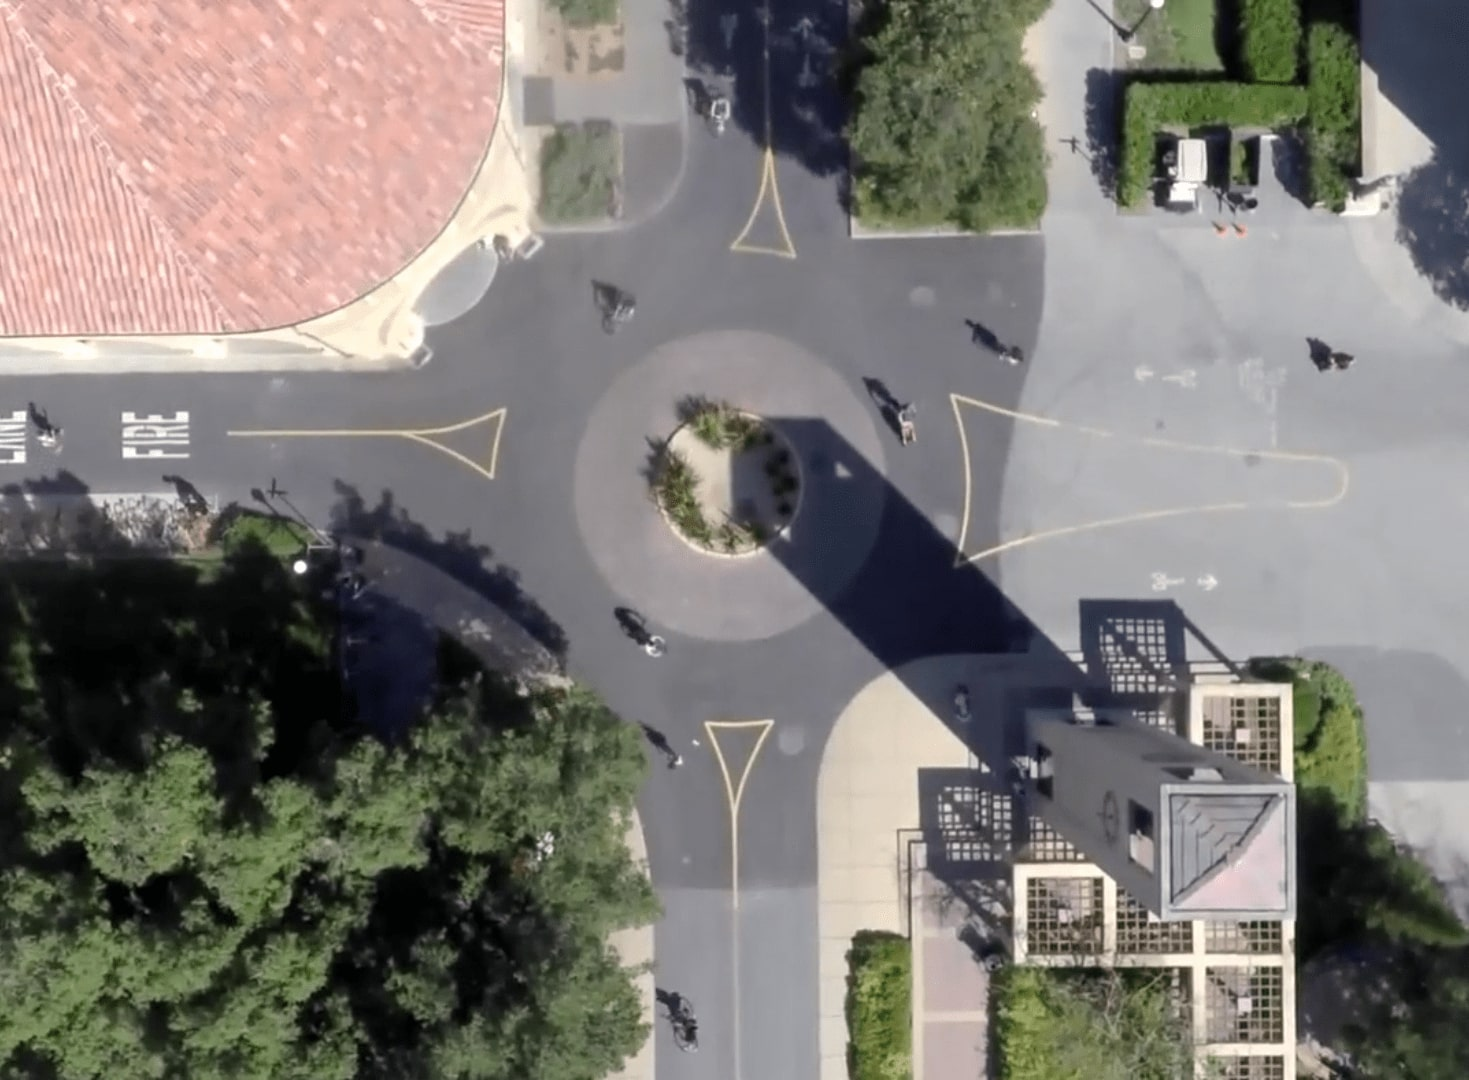
\includegraphics[width=.49\textwidth]{res-death_circle-4.jpg} \\
    \end{tabular}
    \caption[Otestování algoritmu na scéně Death Circle]{Vstupní 5~vteřinové video ze scény Death Circle. Záznam je podobného typu jako ze scény Little. V~záběrech se objevují cyklisté a chodci, procházejí skrz stíny, případně pod zákryty stromů.}
\end{figure}

\begin{figure}[H]
    \centering
    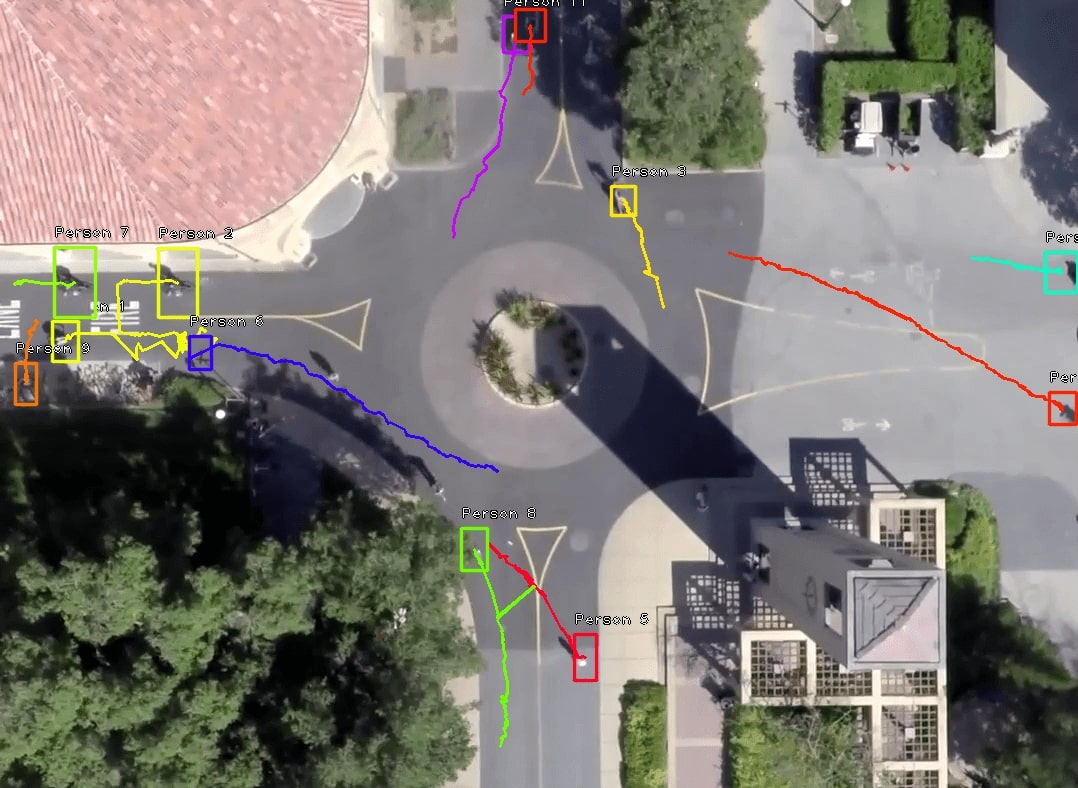
\includegraphics[width=.99\textwidth]{res-death_circle-panorama.jpg}
    \caption[Výsledná mapa s~trajektoriemi osob ze scény Death Circle]{Výsledná mapa s~trajektoriemi osob ze scény Death Circle.}
\end{figure}

Ve spodní části videa jdou proti sobě lidé označeni čísly~5 a~8. Osoba~8 se na krátký okamžik detektoru ztratí. Jako nejbližší a nejpodobnější detekce je pak vyhodnocena osoba~5, proto ta zelená linie k~červené. V~pravé horní části obrazu se vyskytuje 5~osob, jejichž detekce i predikce trajektorií je bezchybná. V~levé části jede mimo záznam cyklista~2 a proti němu cyklista~1, později identifikován jako cyklista~6. V~momentě, kdy si jsou nejblíže, nastává pro cyklistu~2 zmatek a jeho trajektorie uhýbá směrem k~cyklistovi~1. O~několik snímků později je cyklista~2 identifikován jako cyklista~7 a dále je jeho pohyb zaznamenán správně. Cyklista~1 je od doby, co není zaměňován s~cyklistou~2 identifikován jako cyklista~6 a jeho trajektorie je také vizualizována správně. V~této části se nachází ještě osoba~9, pro kterou je detekce korektní.

%-------------------------------------------------------------------------------

\subsection*{První scéna z~natáčení dronem}

Pro další experimentování a vyhodnocování úspěšnosti byly pořízeny záběry dronem DJI Spark. Skupinka osob se náhodně pohybovala po natáčeném prostoru. Vzniklo několik záběrů, které byly následně sestříhány a využity pro další otestování algoritmu. Hranice, pro vyhodnocení detekce neuronovou sítí jako úspěšné, byla snížena z~výchozí hodnoty~0,5 na~0,4.

\begin{figure}[H]
    \begin{tabular}{cc}
        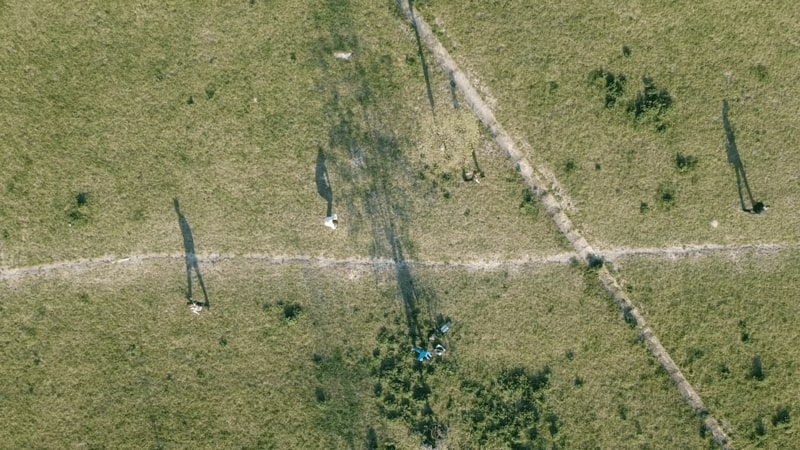
\includegraphics[width=.49\textwidth]{res-drone-vid1-1.jpg} &
        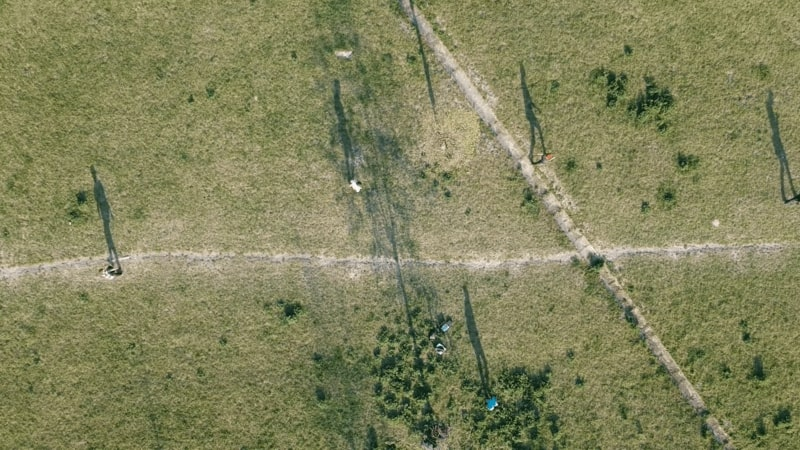
\includegraphics[width=.49\textwidth]{res-drone-vid1-2.jpg} \\
        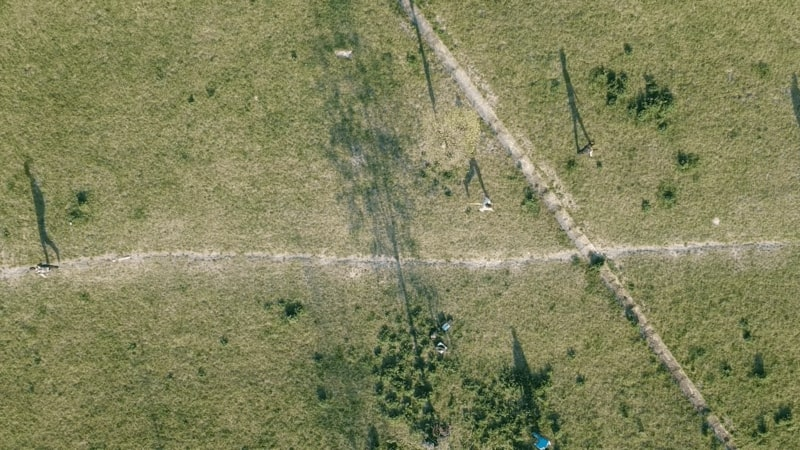
\includegraphics[width=.49\textwidth]{res-drone-vid1-3.jpg} &
        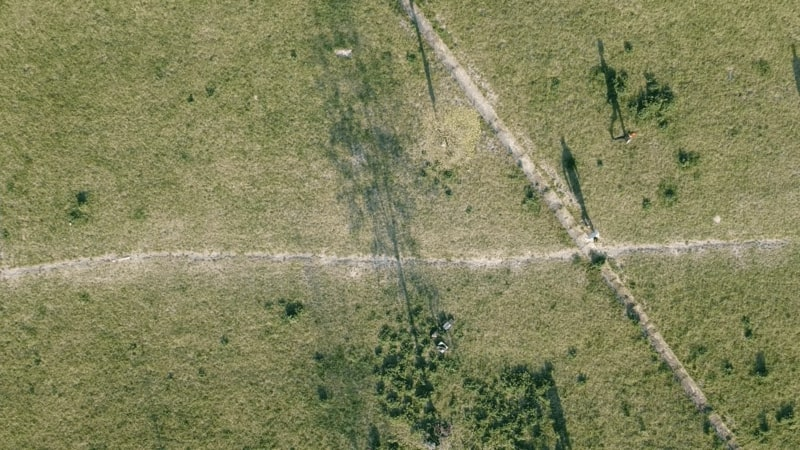
\includegraphics[width=.49\textwidth]{res-drone-vid1-4.jpg} \\
    \end{tabular}
    \caption[Otestování algoritmu na prvním záznamu z~dronu]{Vstupní 6~vteřinové video. První záznam pořízený dronem. Na počátku je v~obraze 5~lidí a postupně všichni odcházejí mimo záběr.}
\end{figure}

\begin{figure}[H]
    \centering
    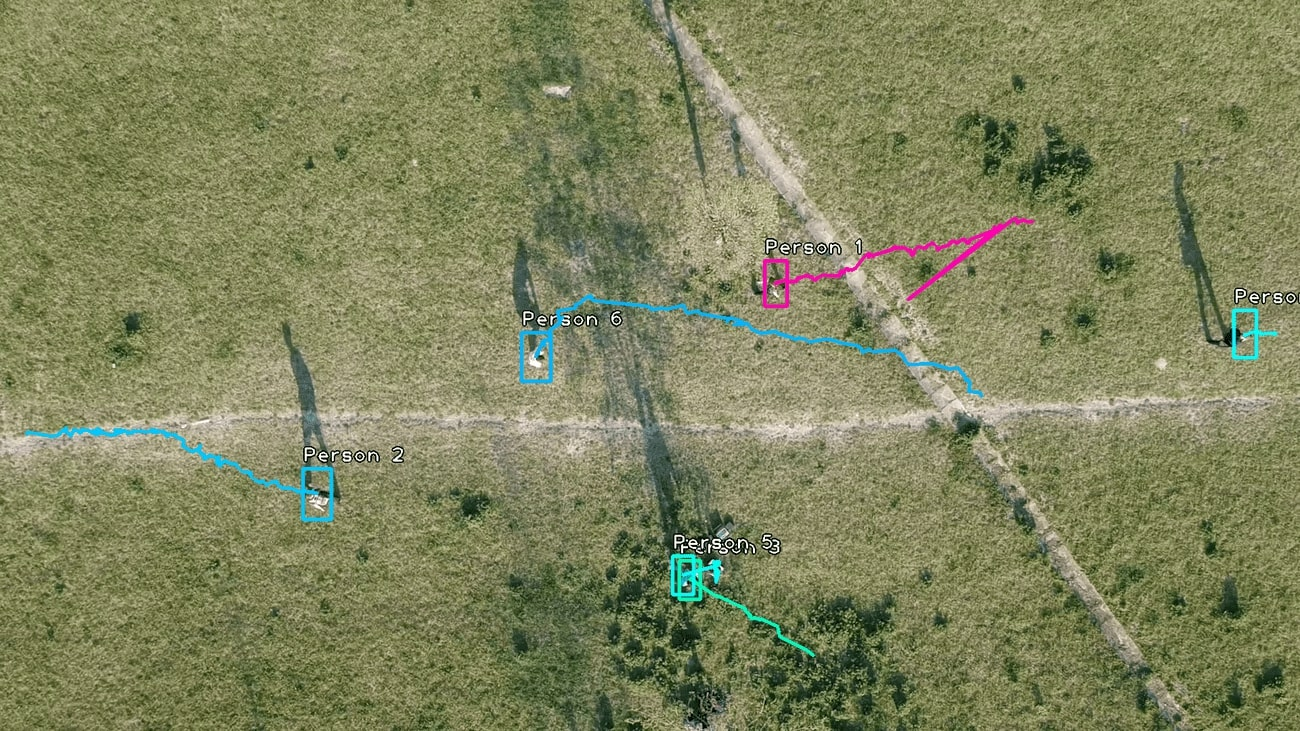
\includegraphics[width=.99\textwidth]{res-drone-vid1-panorama.jpg}
    \caption[Výsledná mapa s~trajektoriemi osob z~první scény]{Výsledná mapa s~trajektoriemi osob z~první scény.}
\end{figure}

Všechny osoby byly v~průběhu záznamu detekovány a jejich trajektorie zakresleny. Osoba~1 byla ke konci mylně spojena s~jiným bodem. Pravděpodobně síť osobu na moment ztratila a zároveň rozpoznala jiný bod jako člověka o~kus vedle. Osoba~5 a~3 jsou na počátku detekováni jako dvě osoby, jedná se pouze o~jednu. Zbytek reidentifikací a vykreslení trajektorií je správné.

%-------------------------------------------------------------------------------

\subsection*{Druhá scéna z~natáčení dronem}

\begin{figure}[H]
    \begin{tabular}{cc}
        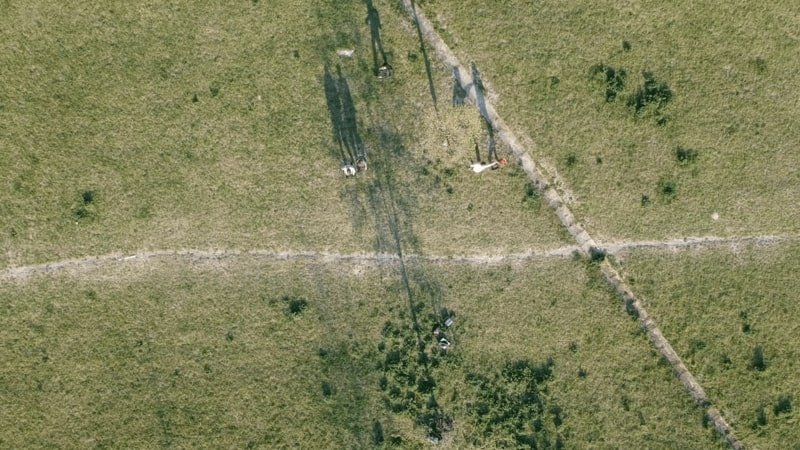
\includegraphics[width=.49\textwidth]{res-drone-vid2-1.jpg} &
        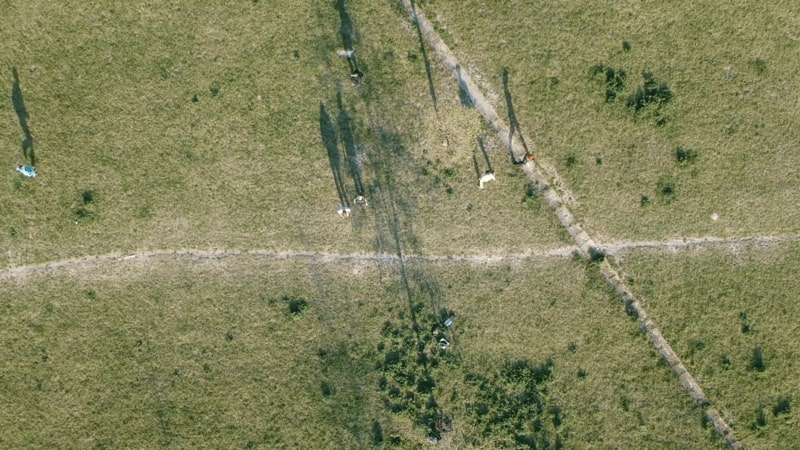
\includegraphics[width=.49\textwidth]{res-drone-vid2-2.jpg} \\
        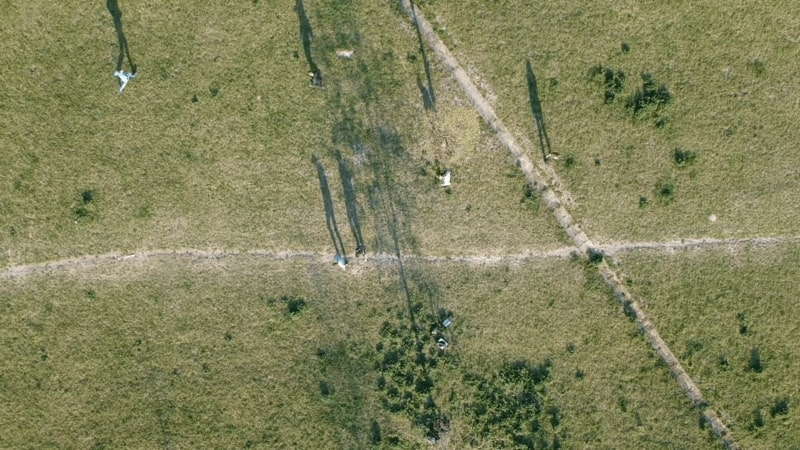
\includegraphics[width=.49\textwidth]{res-drone-vid2-3.jpg} &
        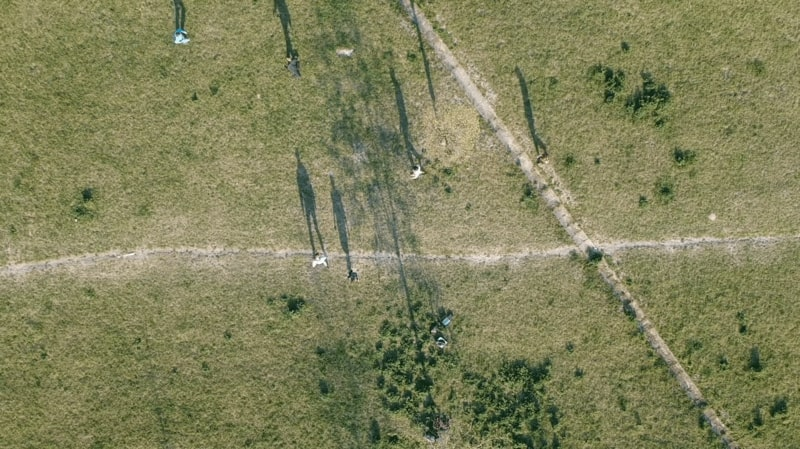
\includegraphics[width=.49\textwidth]{res-drone-vid2-4.jpg} \\
    \end{tabular}
    \caption[Otestování algoritmu na druhém záznamu z~dronu]{Vstupní 5~vteřinové video. Druhý záznam pořízený dronem. 6~osob pohybujících se v~záběru.}
\end{figure}

\begin{figure}[H]
    \centering
    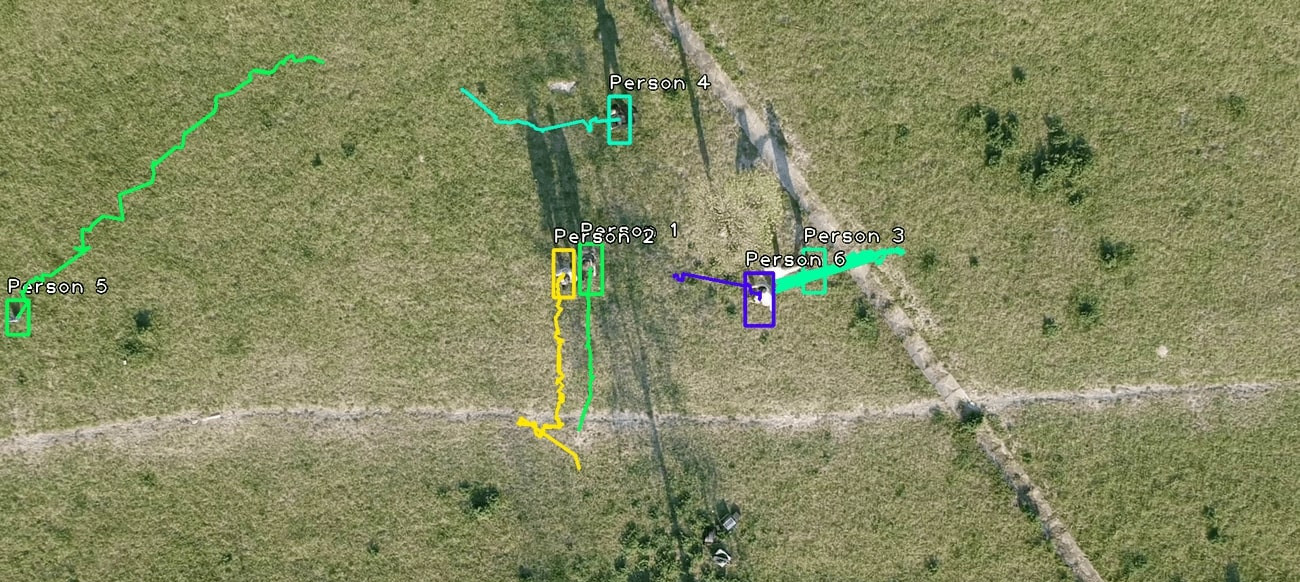
\includegraphics[width=.99\textwidth]{res-drone-vid2-panorama.jpg}
    \caption[Výsledná mapa s~trajektoriemi osob z~druhé scény]{Výsledná mapa s~trajektoriemi osob z~druhé scény.}
\end{figure}

Lidé~1 a~2 jdou vedle sebe, jsou od sebe správně rozlišeni na základě vektoru příznaků a jejich trajektorie jsou korektně vykresleny. Osoby~6 a~3 běží od sebe. 6~je rozpoznána až později, nejdřívě je několikrát mylně zaměněna s~osobou~3. Výsledkem je několik dlouhých, rovných linií. Lidé~5 a~4 jsou reidentifikovány po celou dobu správně a jejich trajektorie jsou korektní.

%===============================================================================
